
\documentclass[reprint,english,notitlepage,aps,nobalancelastpage,nofootinbib]{revtex4-1}  % defines the basic parameters of the document
% if you want a single-column, remove reprint

% allows special characters (including æøå)
\usepackage[utf8]{inputenc}
%\usepackage [norsk]{babel} %if you write norwegian
\usepackage[english]{babel}  %if you write english
\usepackage[T1]{fontenc}


%% note that you may need to download some of these packages manually, it depends on your setup.
%% I recommend downloading TeXMaker, because it includes a large library of the most common packages.

\usepackage{physics,amssymb}  % mathematical symbols (physics imports amsmath)
\usepackage{graphicx, bm}         % include graphics such as plots
\usepackage{upgreek}
\usepackage{float}
\usepackage{xcolor}           % set colors
\usepackage[hidelinks]{hyperref}         % automagic cross-referencing (this is GODLIKE)
\usepackage{tikz}             % draw figures manually
\usepackage{listings}         % display code
\usepackage{subfigure}        % imports a lot of cool and useful figure commands
\usepackage{verbatim}
\usepackage{adjustbox}
\usepackage{mathpazo}
\usepackage{siunitx}
\usepackage{kantlipsum}
\usepackage{bigints}
\usepackage{multirow}
\usepackage{geometry}
\usepackage{algorithm2e}
\usepackage{amsmath}

% defines the color of hyperref objects
% Blending two colors:  blue!80!black  =  80% blue and 20% black
\hypersetup{ % this is just my personal choice, feel free to change things
    colorlinks,
    linkcolor={red!50!black},
    citecolor={blue!50!black},
    urlcolor={blue!80!black}}

%% Defines the style of the programming listing
%% This is actually my personal template, go ahead and change stuff if you want
\lstset{ %
	inputpath=,
	backgroundcolor=\color{white!88!black},
	basicstyle={\ttfamily\scriptsize},
	commentstyle=\color{magenta},
	language=Python,
	morekeywords={True,False},
	tabsize=4,
	stringstyle=\color{green!55!black},
	frame=single,
	keywordstyle=\color{blue},
	showstringspaces=false,
	columns=fullflexible,
	keepspaces=true}

\newcommand\numberthis{\addtocounter{equation}{1}\tag{\theequation}}
\newcommand{\ihat}{\boldsymbol{\hat{\textbf{\i}}}}
\newcommand{\jhat}{\boldsymbol{\hat{\textbf{\j}}}}
\newcommand{\khat}{\boldsymbol{\hat{\textbf{k}}}}
\newcommand{\del}[1]{\textbf{#1)}}
\newcommand{\svar}[1]{\underline{\underline{{#1}}}}
\newcommand{\vc}[1]{\mathbf{#1}}
\renewcommand{\deg}{^{\circ}}
\newcommand{\hksqrt}[2][]{\ \mathpalette\DHLhksqrt{[#1]{#2\,}}}
\def\DHLhksqrt#1#2{\setbox0=\hbox{$#1\sqrt#2$}\dimen0=\ht0
	\advance\dimen0-0.3\ht0
	\setbox2=\hbox{\vrule height\ht0 depth -\dimen0}
	{\box0\lower0.65pt\box2}}

\newcommand{\expy}{\mathbb{E}[\mathbf{\tilde{y}}]}
\newcommand{\expz}{\mathbb{E}[\mathbf{\tilde{z}}]}
\newcommand{\closed}[1]{\left({#1}\right)}
\newcommand{\bracket}[1]{\left[{#1}\right]}


\graphicspath{{../output/plots/}} % search for figures in this dir



\begin{document}


\begin{titlepage}
	\begin{center}
	\textbf{Analysis of Regression and Resampling Methods}

	\vspace{0.2cm}
	Håkon Olav Torvik, Vetle Vikenes and Sigurd Sørlie Rustad

	\vspace{0.5cm}
	
\includegraphics[scale=0.5]{../../pictures/UIO}
	\vspace{0.8cm}

	University of Oslo\\
	Norway\\
	\today	\\
	\end{center}
	\tableofcontents
	\clearpage
\end{titlepage}
%\maketitle                              % creates the title

\onecolumngrid
\section*{Introduction}

Regression analysis is a statistical method for fitting a function to data. It is useful for building mathematical models to explain noisy observations. There are several regression methods to achieve this, all with their strengths and weaknesses. We will in this paper study three different methods; ordinary least squares, Ridge and Lasso regression. All the code, results and instructions on running the code can be found in our GitHub repository\footnote{\href{https://github.com/sigurdru/FYS-STK4155/tree/main/project1}{https://github.com/sigurdru/FYS-STK4155/tree/main/project1}}.

The mathematical model obtained from regression analysis can be used to predict an outcome, given some previously untested input. To build an accurate model, one has to train it on a lot of data. Real-world datasets usually have a fixed size, and getting more data can be practically impossible. By training the model on one particular data set only, we might risk that our model is only efficient for that specific configuration, while predictions made about different data sets will be bad. It is therefore useful to have tools to avoid this for small datasets. Resampling methods are such tools. In addition to the regression methods, we will also study the effect of bootstrapping and cross-validating the data.

In order to study this, we need data to analyze. We will in this paper test the methods on two datasets. We will generate one dataset ourselves using a noisy analytical bivariate function, the Franke function \eqref{eq:FF}, while the other is real-world terrain data. The fitting we will perform for both data sets is a polynomial fit with $x$ and $y$ dependence of the form $[1,\,x,\,y,\,x^2,\,xy,\,y^2,\,\dots]$.

\begin{align}
	\begin{split}\label{eq:FF}
		f(x,y) = &\frac{3}{4}\exp(-\frac{(9x -2)^2}{4} - \frac{(9y-2)^2}{4}) + \frac{3}{4}\exp(-\frac{(9x + 1)^2}{49} - \frac{(9y + 1)}{10})
		\\
		+ &\frac{1}{2}\exp(-\frac{(9x-7)^2}{4} - \frac{(9y -3)}{4}) - \frac{1}{5}\exp(-(9x-4)^2 - (9y-7)^2)
	\end{split}
\end{align}

We will begin by using the simplest regression method, ordinary least squares (OLS), to fit polynomials up to fifth order on the Franke function. At first we will not resample the data, only test our implementation and do some basic analysis. We will then add the resampling methods, Bootstrapping and Cross-Validation, and analyze various quantities from the resulting fits. After that we will do the same analyses as before, but using the more complex regression methods Ridge and Lasso. Having tested different methods on the Franke function, we will repeat these analyses in the end when studying terrain data. This paper will not study the effects of different scaling methods, train-test split ratios and amount of noise.

\section*{Exercise 1: Ordinary Least Square (OLS) on the Franke function}

We generate a dataset drawing $n=30$ uniformly distributed points in $x, y \in[0, 1]$. Equation \eqref{eq:FF} is then used to create $n^2$ \(z\)-values. In this domain, the Franke function takes values \(z\in[-0.45, \hspace{1mm} 1.52]\) before scaling. To this we add normally distributed stochastic noise. The noise has a mean of $\mu=0$, and variance $\sigma^2=1$. It is scaled by a factor $\epsilon$, which we normally set to $\epsilon=0.2$. This gives a substantial amount of noise, without completely drowning out the data. The data with and without noise is visualized in figure \ref{fig:FF_dataset}.

\begin{figure}[h]
	\minipage{0.49\textwidth}
	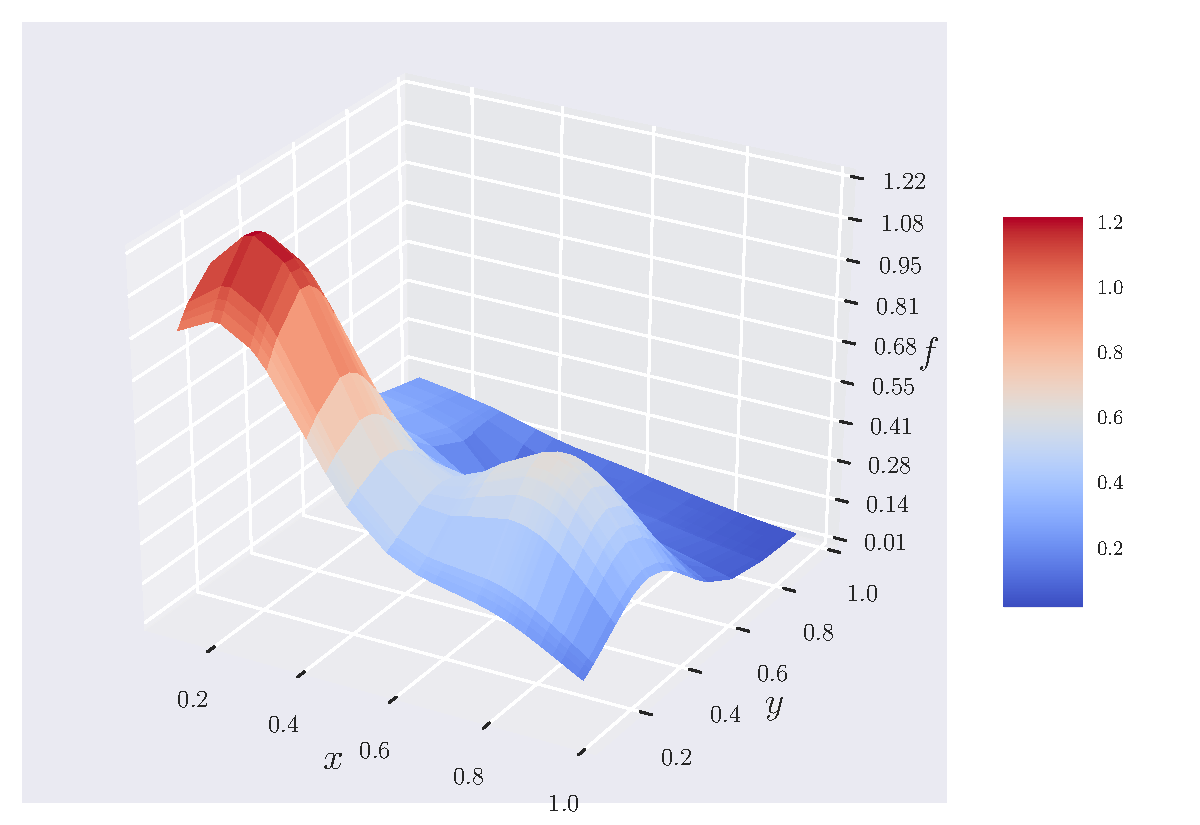
\includegraphics[width=\linewidth]{Frank_anal_eps_0.pdf}
	\endminipage\hfill
	\minipage{0.49\textwidth}
	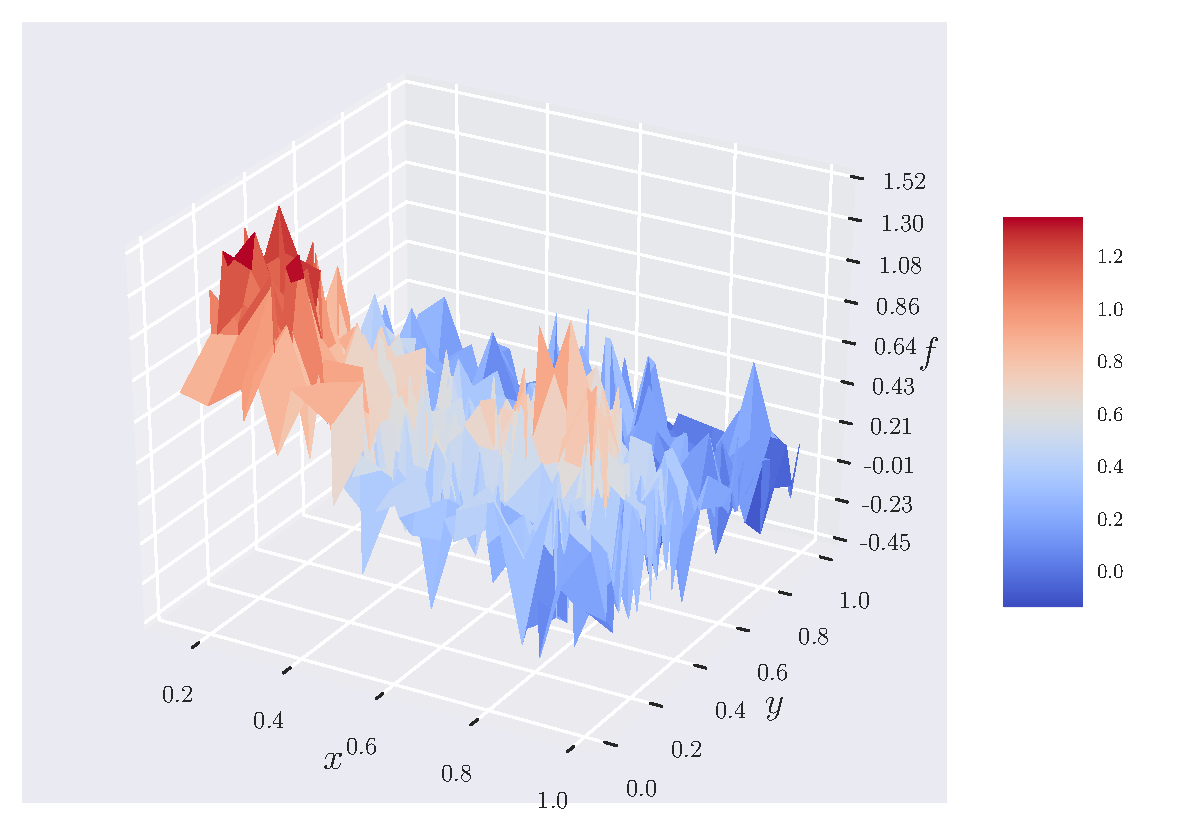
\includegraphics[width=\linewidth]{Franke_rawdata_eps02.pdf}
	\endminipage
	\caption{Here we have displayed our noisy data along with the analytical function. The left figure shows the analytical Franke function, while the right figure is the Franke function with noise.}\label{fig:FF_dataset}
\end{figure}

It is good practice in regression analysis to scale the data, such that different features take values in the same order of magnitude. There are several different methods for scaling, one of which is StandardScaler. This is done by subtracting the mean from the data, before dividing this by the standard deviation. This centres the data around $0$ and sets the variance to $1$. Because our $x$ and $y$ is already in the domain $[0, 1]$ with variance $1$, this only shifts it down, and has no outcome on the regression results. For $z$ generated using \eqref{eq:FF} the effect is small, but we choose to do this for consistency. Our also code allows for the following different scaling methods: no scaling, Normalizer and MinMax, though these will not be used.

One main advantage of scaling the data becomes evident when we consider terrain data later on. The altitude of the terrain could vary hundreds of meters between the lowest and highest point, and if we were to study the errors of our model predictions, we would not necessarily be able to determine whether an error of order $10$ is good or bad. By scaling the data we get the relative error of our prediction, which gives a simpler assessment of the resulting fit.

We are fitting a bivariate polynomial of degree $p$. With $p$ as the highest polynomial degree, the polynomial will have $N_p=(p+1)(p+2) / 2$ terms. It can, without noise, be written
\begin{equation}\label{eq:zpolynm}
	z(x, y) = \beta_0 + \beta_1x + \beta_2y + \beta_3x^2 + \beta_4xy + \beta_5y^2 + \dots
\end{equation}
where the $\beta$-parameters are coefficients for each term. The $x$ and $y$'s are collected in a design matrix $X$. The columns of $X$ are the terms, while the rows are all terms for a single datapoint. $X$ thus have size $(n^2\cross N_p)$. The $\beta$s are collected in a vector $\boldsymbol{\beta}$ of length $p$. These are unknown parameters to be determined.

Thus, out model with stochastic noise takes the form
\begin{equation}
	\label{eq:z_true_data}
	\vc{z} = X \boldsymbol{\beta} + \boldsymbol{\epsilon},
\end{equation}

One challenge in our case is that our data is two-dimensional, i.e. $\vc{z}$ has dimensions $(n,n)$. We create a workaround by mapping our two-dimensional data, to a one dimensional $(n^2,1)$ vector. This is an important note, and we will do this throughout the report.

We want to create a model to predict $\vc{z}$ given an input. $\boldsymbol{\tilde\beta}$ are the optimal parameters obtained from regression. Our prediction \(\boldsymbol{\tilde{\vc{z}}}\) is then given by

\begin{equation*}
	\boldsymbol{\tilde{z}} = X\boldsymbol{\tilde{\beta}}.
\end{equation*}

To asses the quality of the model, we need a way to quantify the error. We will use the mean square error (MSE), and $R^2$-score, given by

{\large
\begin{align*}
	MSE(\boldsymbol{z}, \boldsymbol{\tilde{z}}) &= \frac{1}{N}\sum_{i=0}^{N-1} (z_i - \tilde{z}_i)^2 = \frac{1}{N}\left\{(\vc{z} - X\boldsymbol{\tilde{\beta}})^T(\vc{z} - X\boldsymbol{\tilde{\beta}})\right\}.
	\\
	R^2(\boldsymbol{z}, \boldsymbol{\tilde{z}}) &= 1 - \frac{\sum_{i=0}^{n-1}(z_i - \tilde{z}_i)^2}{\sum_{i=0}^{n-1}(z_i - \bar{z})^2}, \hspace{3mm} \bar{z} = \frac{1}{n}\sum_{i=0}^{n-1}z_i
\end{align*}
}%

MSE will always be larger than 0, and an MSE of 0 means our model fits the data perfectly. Throughout this paper, MSE and error will be used interchangeably. The $R^2$-score is a number between 0 and 1, with 1 being a perfect fit. In order to find the optimal parameters $\boldsymbol{\hat{\beta}}$ we need a cost function to minimize. Choosing MSE as the cost-function gives the expresion for OLS-regression.
\begin{equation*}
	C(\boldsymbol{\beta}) = MSE(\boldsymbol{z}, \boldsymbol{\tilde{z}})
\end{equation*}
Minimizing this is done by doing the derivative with respect to all the parameters, and finding the zero.
\begin{equation}\label{eq:Const_OLS}
	\frac{\partial C(\boldsymbol{\beta})}{\partial \boldsymbol{\beta}} \equiv 0 = X^T(\boldsymbol{z} - X\boldsymbol{\tilde{\beta}}).
\end{equation}
We can rewrite this as
\begin{equation}\label{eq:OLS_beta}
	X^T\vc{z} = X^TX\boldsymbol{\tilde{\beta}} \implies \boldsymbol{\tilde{\beta}} = (X^TX)^{-1} X^T \vc{z} \equiv \boldsymbol{\hat{\beta}}
\end{equation}
This is OLS-regression. Thus $\boldsymbol{\hat{\beta}}$ are the optimal parameters that minimizes the cost function.

Now that we have an expression for the optimal parameters, we also want to evaluate how good our results are. We do this by splitting our data into two sets, one set for training (80\%) and one set for testing (20\%). We can then find the optimal parameters ($\boldsymbol{\hat{\beta}}$) using the train data, and then compare our test data to the actual data.

%There are many quantities we can use to evaluate our results, however we have decided to calculate the MSE and $R^2$ score. MSE is given by equation \eqref{eq:MSE} and the $R^2$ score by equation \eqref{eq:R2}.
%\begin{equation}
%	\label{eq:MSE}
%	MSE(\vc{z}, \vc{\tilde{z}}) = \frac{1}{n}\sum_{i=0}^{n-1}(z_i - \tilde{z}_i)^2
%\end{equation}
%$MSE(\vc{z}, \vc{\tilde{z}})$ is the mean square between the datapoints $\vc{z}$ and $\vc{\tilde{z}}$.
%\begin{equation}
%	\label{eq:R2}
%	R^2(\vc{z}, \vc{\tilde{z}}) =
%\end{equation}
%Here $R^2(\vc{z}, \vc{\tilde{z}})$ is the $R^2$ score between the datapoints $\vc{z}$ and $\vc{\tilde{z}}$.

We can now perform OLS on our data and plot the MSE and $R^2$-score as a function of polynomial degree. It is important to note that when we fit using a polynomial of degree $p$, all terms from lower polynomial degrees are included in the fit. We expect the MSE to strictly decrease and $R^2$ to strictly increase for the train data, as our model becomes more complex. We expect the same for the test data, however at a certain polynomial degree we might se overfitting. This would make our error increase and $R^2$ score decrease. The results are plotted in figure \ref{fig:OLS_R2_and_MSE}. Overfitting is when the model nearly perfectly fits the training data, since it tries to fit specific data points. This results in a poor performance on the test data, as these data points are different from the train data. Splitting the data is thus a way to check whether we are overfitting or not, for data from the same dataset, but which the model has not trained on.

\begin{figure}[h]
	\minipage{0.49\textwidth}
	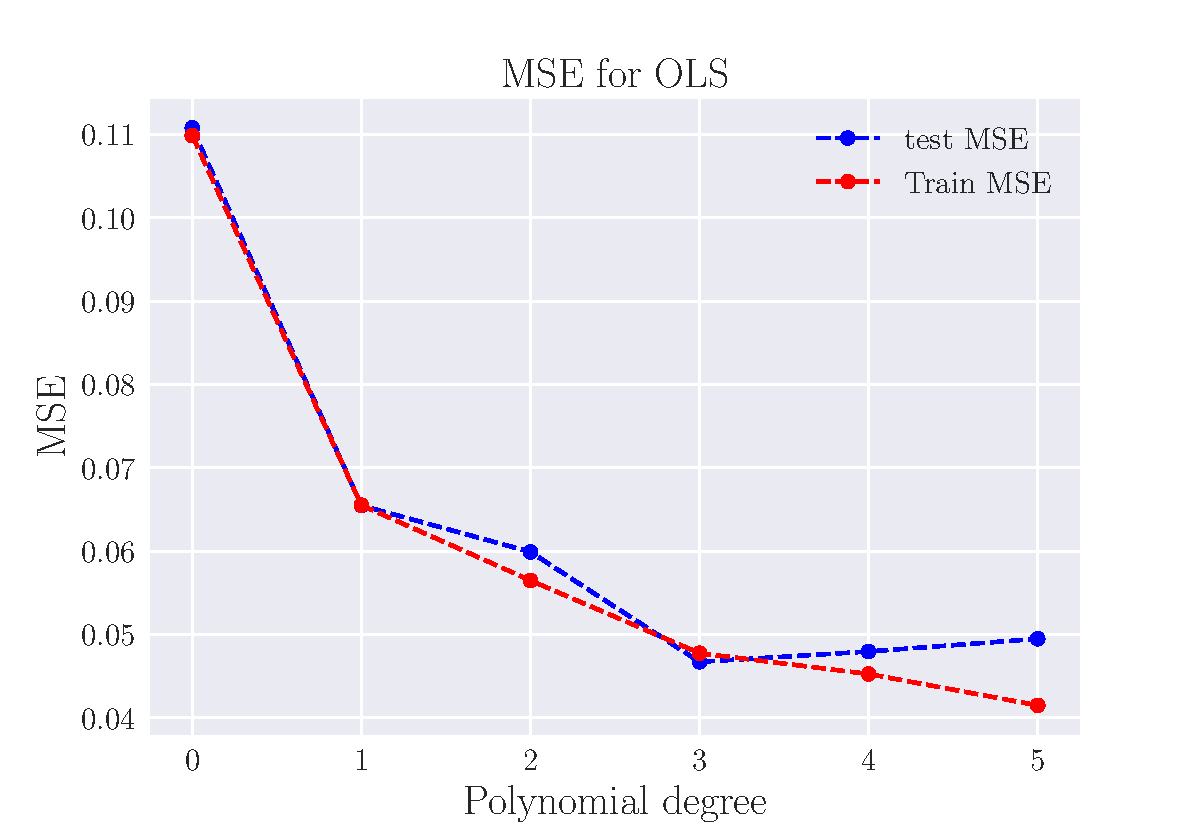
\includegraphics[width=\linewidth]{MSE_OLS_n30_eps02_pol5.pdf}
	\endminipage\hfill
	\minipage{0.49\textwidth}
	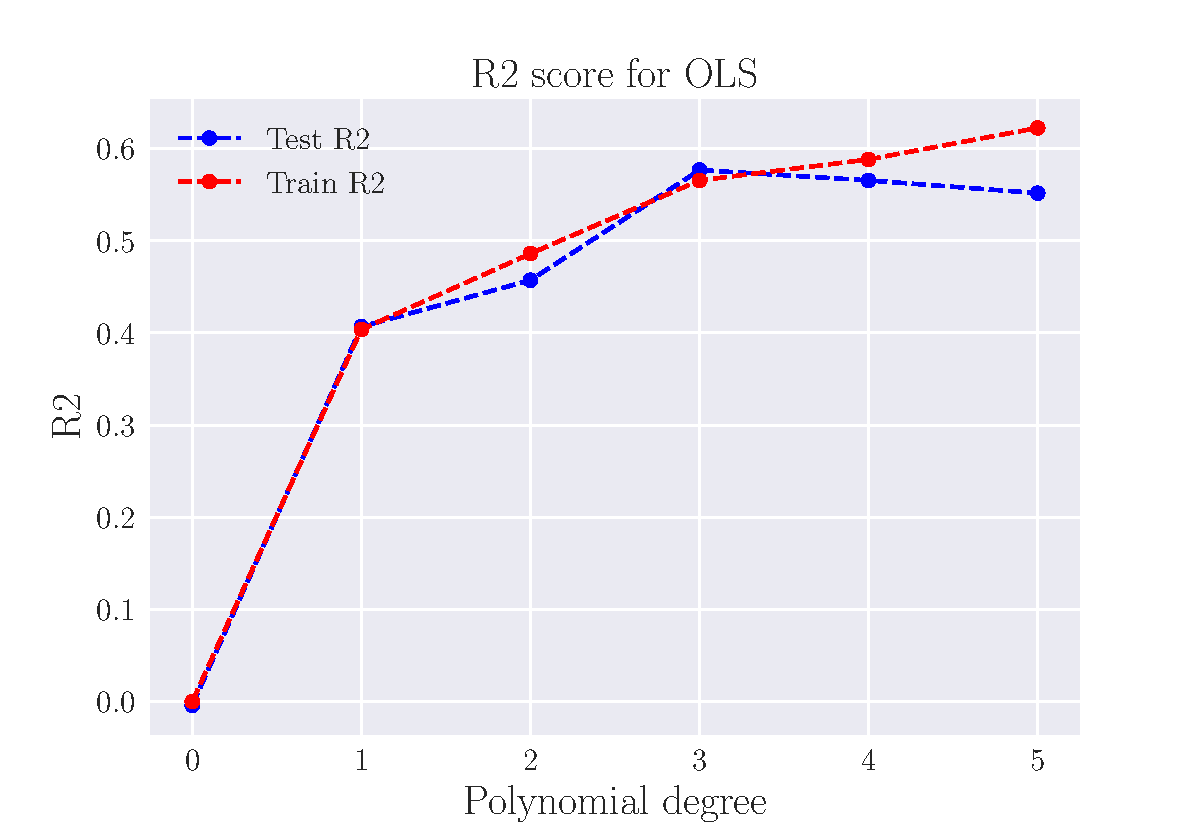
\includegraphics[width=\linewidth]{R2_OLS_n30_eps02_pol5.pdf}
	\endminipage
	\caption{Here we have plotted the MSE and $R^2$-score for OLS. The left figure shows the MSE and right shows the $R^2$ score. The red dotted line is from the train data, and the blue dotted line is from the test data.}\label{fig:OLS_R2_and_MSE}
\end{figure}

From figure \ref{fig:OLS_R2_and_MSE} we see that the MSE strictly decrease and $R^2$-score strictly increase for the train data. For the test data, we see that $p>3$ causes the MSE to increase as well as a reduction of the $R^2$-score. This is an indication that overfitting is starting to occur. The lowest error is $MSE_{min} = 0.0467$, for $p=3$.

It is also interesting to look at the variance in the parameters, because this would give an indication of overfitting. We know that for a set of optimal parameters
$\boldsymbol{\hat{\beta}} = (X^TX)^{-1}X^T \vc{z}$,
We have the expectation value
\begin{equation*}
	\mathbb{E}[\boldsymbol{\hat{\beta}}] = \mathbb{E}[(X^TX)^{-1}X^T \vc{z}] = (X^TX)^{-1}X^T\mathbb{E}[\vc{z}] = (X^TX)^{-1}X^TX\boldsymbol{\hat{\beta}} = \boldsymbol{\hat{\beta}}.
\end{equation*}
With this we can calculate the variance in $\boldsymbol{\hat{\beta}}$.
\begin{align*}
	\text{Var}(\boldsymbol{\hat{\beta}}) &= \mathbb{E}\left[(\boldsymbol{\hat{\beta}} - \mathbb{E}[\boldsymbol{\hat{\beta}}])(\boldsymbol{\hat{\beta}} - \mathbb{E}[\boldsymbol{\hat{\beta}}])^T\right] \\
	&= \mathbb{E}\left[((X^TX)^{-1}X^T\vc{z}- \boldsymbol{\hat{\beta}})((X^TX)^{-1}X^T\vc{z}- \boldsymbol{\hat{\beta}})^T\right] \\
	&= (X^TX)^{-1}X^T \mathbb{E}\left[\vc{z}\vc{z}^T\right]X(X^TX)^{-1}- \boldsymbol{\hat{\beta}}\boldsymbol{\hat{\beta}}^T \\
	&= (X^TX)^{-1}X^T\left[X\boldsymbol{\hat{\beta}}\boldsymbol{\hat{\beta}}^TX^T + \sigma^2 \right] X (X^TX)^{-1} - \boldsymbol{\hat{\beta}}\boldsymbol{\hat{\beta}}^T \\
	&= \boldsymbol{\hat{\beta}}\boldsymbol{\hat{\beta}}^T + \sigma^2(X^TX)^{-1} - \boldsymbol{\hat{\beta}}\boldsymbol{\hat{\beta}}^T = \sigma^2(X^TX)^{-1}
\end{align*}
Here we used $\mathbb{E} (\vc{z}\vc{z}^T) = X \boldsymbol{\hat{\beta}}\boldsymbol{\hat{\beta}}^T X^T + \sigma^2\mathbb{1}$, where $\sigma^2 = \epsilon = 0.2$ is the variance of the noise and $\mathbb{1}$ is the identity matrix. Now we have an estimate for the variance in parameter $\boldsymbol{\hat{\beta}}_{j}$ given by
\begin{equation}
	\boldsymbol{\sigma}^2(\boldsymbol{\hat{\beta}}_{j}) = \sigma^2 [(X^TX)^{-1}]_{jj}.
	\label{eq:var_OLS}
\end{equation}
where $j$ corresponds to the coefficient, as in equation \eqref{eq:zpolynm}. Using equation \eqref{eq:var_OLS} we can plot the confidence interval for the different parameters, for several polynomial degrees (see figure \ref{fig:var_beta}).
\begin{figure}[h]
	\minipage{0.49\textwidth}
	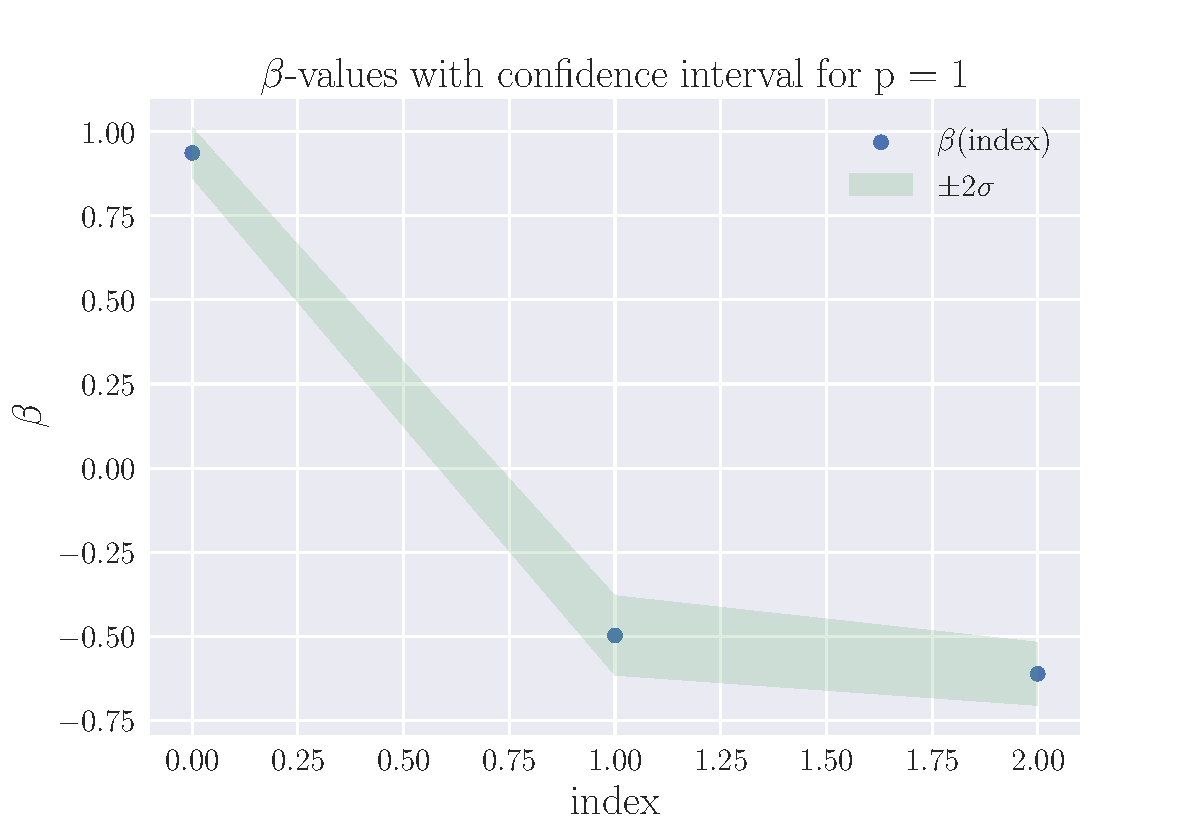
\includegraphics[width=\linewidth]{Var_OLS_poldeg_1.pdf}
	\endminipage\hfill
	\minipage{0.49\textwidth}
	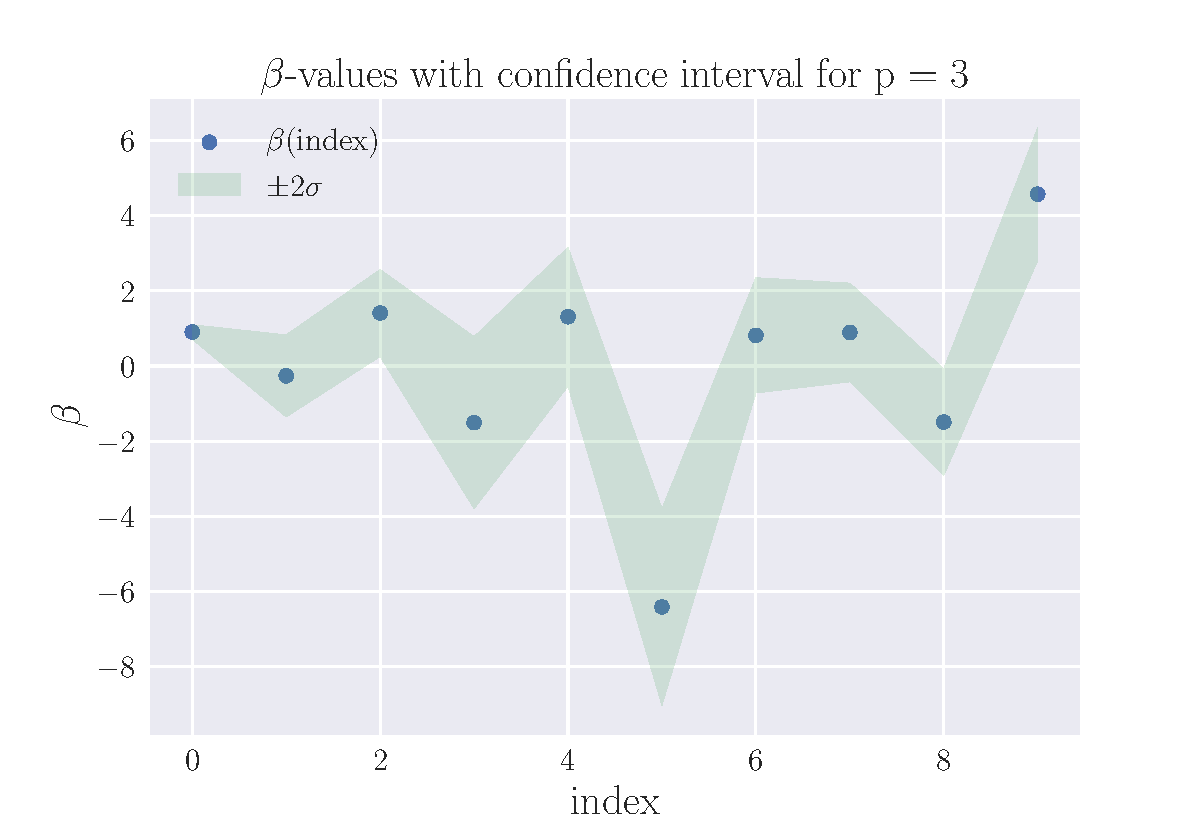
\includegraphics[width=\linewidth]{Var_OLS_poldeg_3.pdf}
	\endminipage\hfill
	\minipage{0.49\textwidth}
	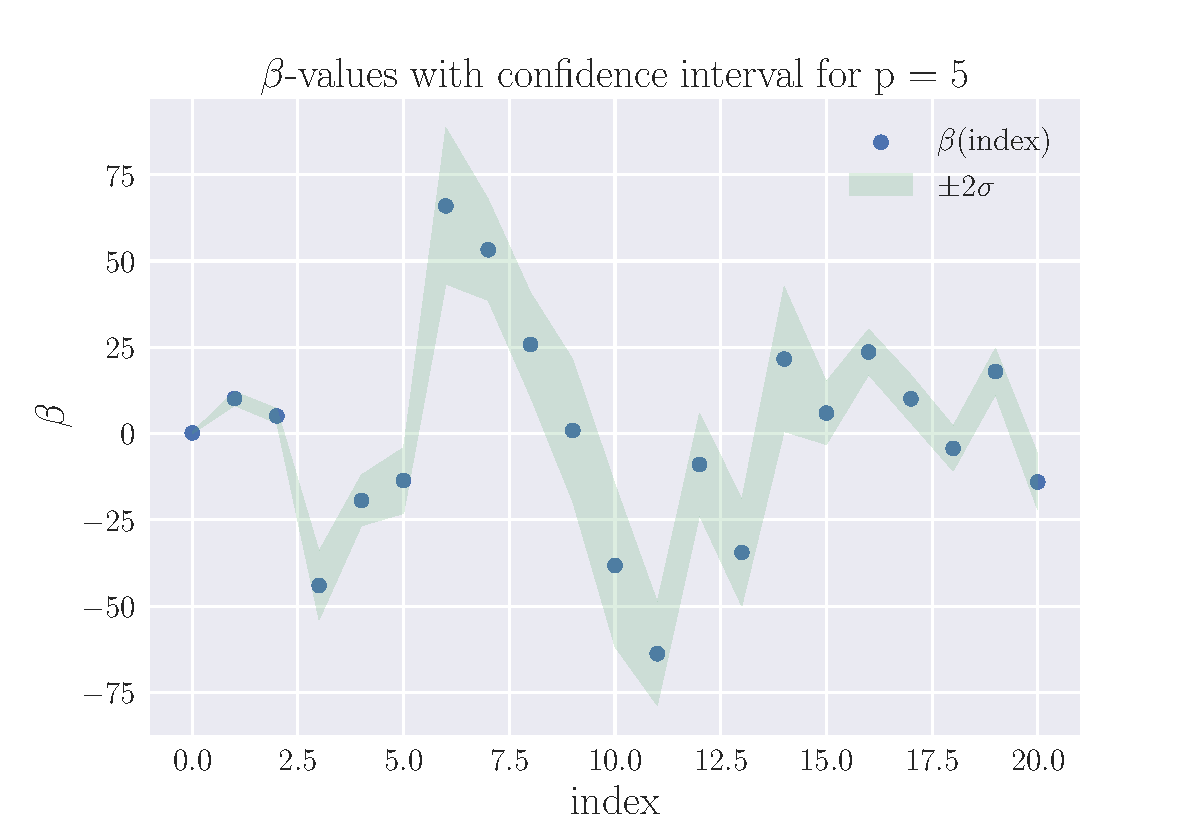
\includegraphics[width=\linewidth]{Var_OLS_poldeg_5.pdf}
	\endminipage\hfill
	\minipage{0.49\textwidth}
	\caption{Here we have plotted the ideal parameters, for different polynomial degrees and with the confidence intervals. Top left figure has polynomial degree $p = 1$, top right $p = 3$ and bottom left $p = 5$. All the plots are of $\boldsymbol{\beta}$ as a function of the index in the vector. The confidence interval is $\pm 2\boldsymbol{\sigma}(\boldsymbol{\hat{\beta}}_{j})$, where $\boldsymbol{\sigma}(\boldsymbol{\hat{\beta}}_{j})$ is given by equation \eqref{eq:var_OLS}.} \label{fig:var_beta}
	\endminipage
\end{figure}
We see in figure \ref{fig:var_beta} that the variance increases as a function of $p$. This is expected because we should get overfitting for higher polynomial degrees\footnote{A discussion of the variance is given in the next section}. For larger $p$ we also have more parameters to tune. This means that an adjustment of one parameter could be compensated by tuning the other parameters in the vicinity. We can see the result of this in the bottom left plot in figure \ref{fig:var_beta}. We observe a large variance in the middle, where we have a high density of parameters, and a lower variance on the edges. One also notices a comparatively low variance for the first parameter $\beta_0$, because of the fixed intercept.


\section*{Exercise 2: Bias-variance trade-off and bootstrapping}

Here we want to evaluate OLS using bootstrapping as a resampling technique. Bootstrap is a way of simulating having more data than you actually have, by reusing the same data. Let's say you have $N$ datapoints, then for every bootstrap-iteration, you would draw $1$ of the $N$ points at random, put it back again and continue until you have drawn a total of $N$ points again. After that you perform the regression analysis. This process is repeated $B$ times. By placing back the datapoints, you would in many cases use the same datapoint several times, even in the same regression. This random sampling will allow us to use a different set of training data in each simulation, without actually having new data, and still reduce the amount of overfitting compared with training on the same data over and over.

Now, with bootstrapping, we want to take a look at when we get overfitting. It is common to see overfitting when we have a high polynomial degree ($p_\text{max}$) compared to the number of datapoints. In figure \ref{fig:OLS_overfitting} we have plotted the test and train MSE for $p_\text{max} = 20$, using $B=90$ resampling iterations. Now, the plotted MSE corresponds to the mean MSE from $90$ iterations for each polynomial degree. The left plot shows the train-error being substantially higher than the test-error, indication of overfitting, for polynomial degrees $p > 7$. On the right panel we have displayed the MSE for $p_\text{max} = 10$, which suggests the beginning of overfitting for $p>3$, and looks very similar to the MSE obtained without bootstrapping from figure \ref{fig:OLS_R2_and_MSE}. This indicates that the MSE we got without bootstrapping was very close to the expected value for $p=2$.

The lowest MSE we got was $MSE_{min}=0.0474$, for $p=3$. This is slightly higher than what we got without resampling. This is because the bootstrap-MSE is a mean of $B$ errors, fluctuating around a value. A different random draw of the noise might have yielded lower MSE for bootstrapping. Increasing the number of bootstrap iterations to $B>90$ yielded no noticeable change in the MSE. Using $B=300$ only changed the MSE in the 7th decimal place. An important point to consider is that despite an increase in the test MSE for $p>3$, the increase is of a relatively low value. This means that a polynomial degree of $p=5$ or $p=7$ could be the best fit for reproducing the Franke function, but $p=3$ happens to yield the lowest MSE for our particular test data, which might be affected by the noise at certain points.

\begin{figure}[h]
	\minipage{0.49\textwidth}
	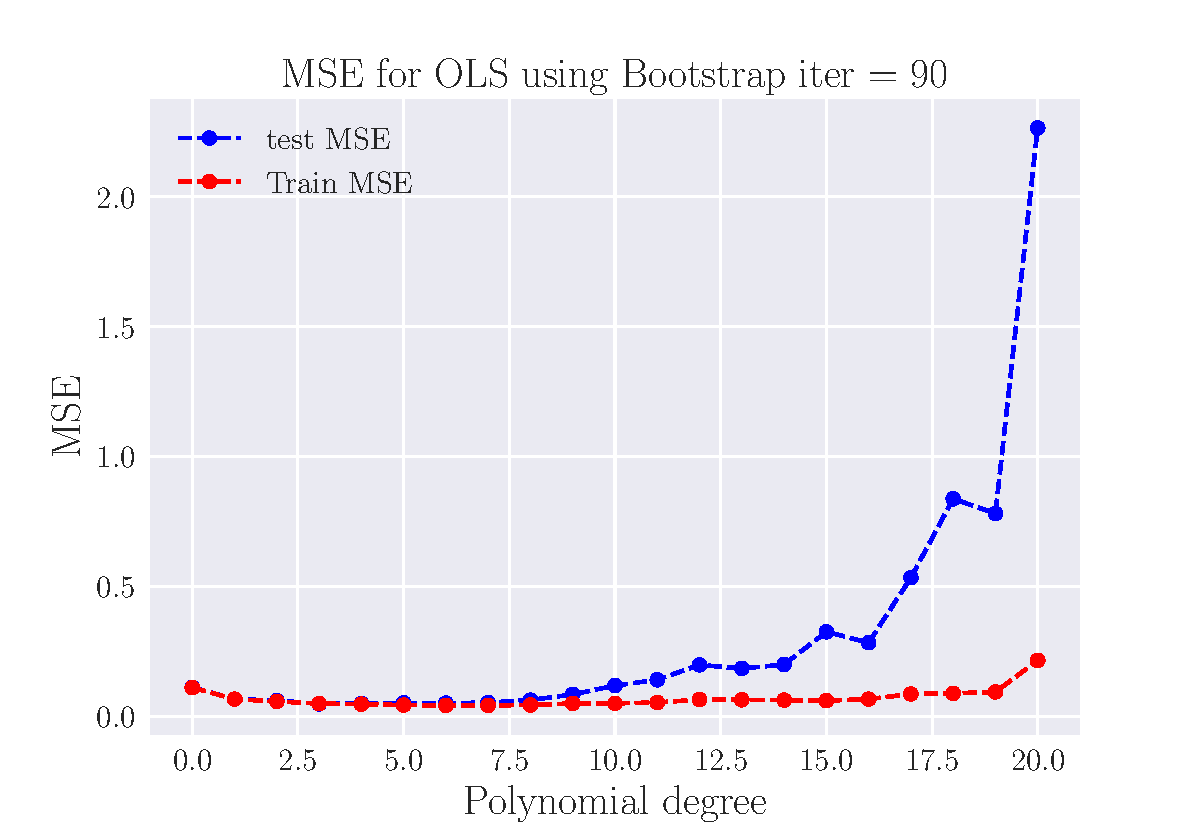
\includegraphics[width=\linewidth]{MSE_OLS_n30_eps02_pol20_Bootstrap_re90.pdf}
	\endminipage\hfill
	\minipage{0.49\textwidth}
	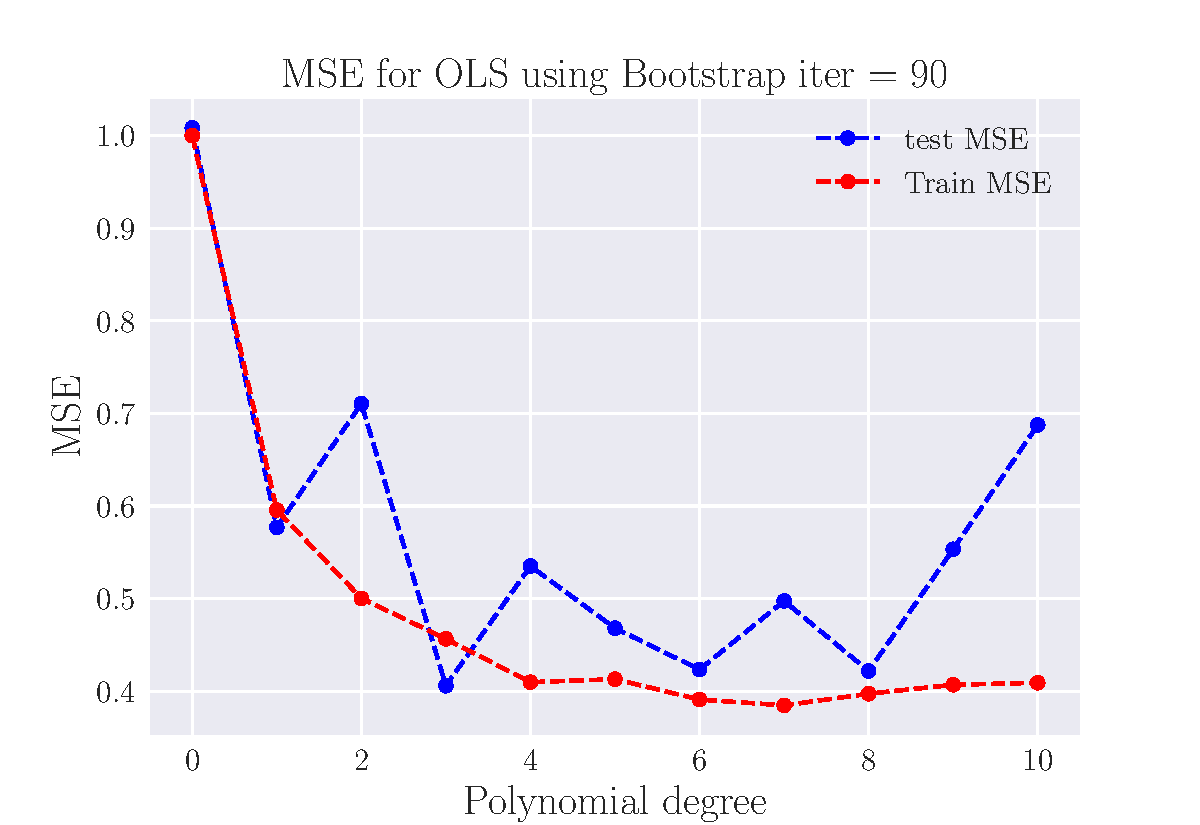
\includegraphics[width=\linewidth]{MSE_OLS_n30_eps02_pol10_Bootstrap_re90.pdf}
	\endminipage
	\caption{Test MSE for OLS with $B=90$ iterations with the Bootstrap resampling method, using $p_\text{max}=20$ on the left panel and $p_\text{max}=10$ on the right panel.}
  \label{fig:OLS_overfitting}
\end{figure}

Before we study the bias variance trade-off, we will take a look at the mathematical expressions. With our data model given in equation \eqref{eq:z_true_data} we find our model by considering the cost function, given as
\begin{align*}
  C(\bm{\beta}) &= \frac{1}{N} \sum_{i=0}^{N-1} (z_i - \tilde{z}_i)^2 = \mathbb{E}[(\mathbf{z}-\mathbf{\tilde{z}})^2]
\end{align*}
where $\mathbb{E}$ is the expected value. % Sample value

We can show that this can be written as\footnote{The derivation is given in Appendix \ref{Apx:BVT}}

\begin{align}
\label{eq:bias_var_tradeoff}
  \mathbb{E}[(\mathbf{z}-\mathbf{\tilde{z}})^2] &= \frac{1}{N}\sum_i (f_i - \expz)^2 + \frac{1}{N}\sum_i (\tilde{z}_i - \expz)^2 + \sigma^2
\end{align}
where $f_i$ is the true data value at point $i$, and $\sigma^2$ the standard deviation of the noise.

In equation \eqref{eq:bias_var_tradeoff} the first term represents the square of the bias, the second term represents the variance while the last term represents the variance of the irreducable error $\epsilon$. When performing linear regression the variance is a measurement on how much our model changes with different training sets. High variance will therefore occur if a different training set resulted in very different values of the individual estimators, $\bm{\hat{\beta}}_j$. This will be the case for overfitting when our model is essentially trying to reproduce variations from the noise. The bias provides information about the difference between our model and the true data values. If our model is missing out on underlying structures in our data we would get a high bias. High bias will thus be the case for an underfitted model. Our goal is therefore to minimize the bias and variance in our model.

Using equation \eqref{eq:bias_var_tradeoff} we can plot the bias, variance and MSE for the test and train data, using the bootstrap method. For both datasets we expect the bias and MSE to start high and variance to start low. For the train data we should get a strictly better fit for higher polynomial degree, making both the bias and MSE to decrease. For the testing data however, when we start to see overfitting the variance and error should increase, while the bias stays low. In figure \ref{fig:BV_OLS} we have plotted bias, variance and MSE for the test and train data, using $B = 90$ resampling iterations. We plot for $p_\text{max} = 15$, to obtain the desired result that the variance should surpass the bias.

\begin{figure}[h]
	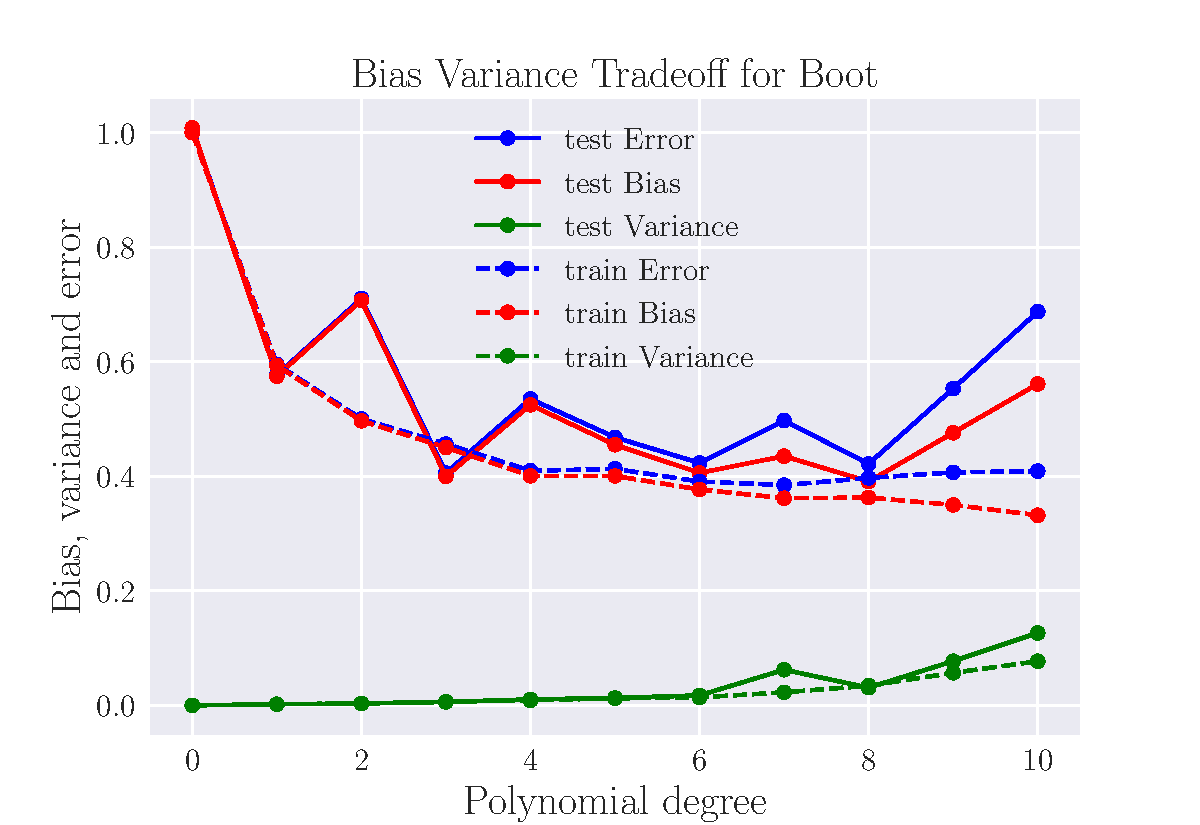
\includegraphics[width=\linewidth]{BVT_OLS_n30_eps0_2.pdf}
	\caption{Here we have plotted the bias, variance and MSE for the test and train data. The $x$-axis shows the polynomial degree, and the $y$-axis indicates the bias, variance and MSE. The dotted lines are for the train data and solid lines are the test data.}\label{fig:BV_OLS}
\end{figure}

As expected we se a general increase in MSE and variance for the test data when the complexity increases, despite a certain dip around $p=13$. The test bias does not act completely as expected. It does decrease in the beginning, however it starts increasing at around $p = 15$. This is likely due to unpredictable behaviour of our model, which we would expect for such a high polynomial degree. The decrease of the MSE and variance also suggests that the model does not behave ideally at all values of $p$. When increasing the number of iterations to $B=300$, the MSE and variance kept increasing up to $p=14$, while they dipped at $p=15$. The increase of the test bias at $p=15$ was reduced as well, causing it to end up with a final value below $0.10$. This suggests that our model behaves somewhat unpredictable at sufficiently high polynomial degree, but other than that, the results are just as we expected. We were also able to see that the variance surpasses the bias for sufficiently high model complexity.

As previously discussed, the minimum value of the test MSE at $p=3$ does not seem to correspond to the best fit, according to our bias-variance trade-off analysis. There seems to be a slight increase in variance at $p=7$, which is also the case for the test MSE. Taking all of this into account, the optimal fit of the Franke function that minimizes bias, variance and MSE for OLS appears to be either $p=6$ or $p=7$ with bootstrap resampling. Considering the low test MSE we got for $p=3$, our results depend on the particular test data we use. Making a final conclusion about whether $p=6$ or $p=7$ gives the best prediction would therefore be more appropriate if we had studied the bootstrap method for different sets of test data, which we have not done. This could give an indication about the validity of the differences between the two polynomial degrees.


\section*{Exercise 3: Cross-validation as resampling technique, adding more complexity}

Here we have implemented cross-validation as the resampling technique. This works by first shuffling the data randomly, then split the data into $k$ different groups. We choose one group to be the test-data and perform linear regression with the remaining data as the training set. The MSE is calculated with the test data. We then choose a new group to be the test data and calculate the MSE once again with the remaining groups as the training data. We repeat the process a total of $k$ timer, until all the groups have been used as test data exactly once. The final MSE will then be the mean MSE, after all the iterations. In figure \ref{fig:CV_OLS} we have performed cross-validation resampling, using $k = [5,7,10]$ iterations.

\begin{figure}[h]
	\minipage{0.49\textwidth}
	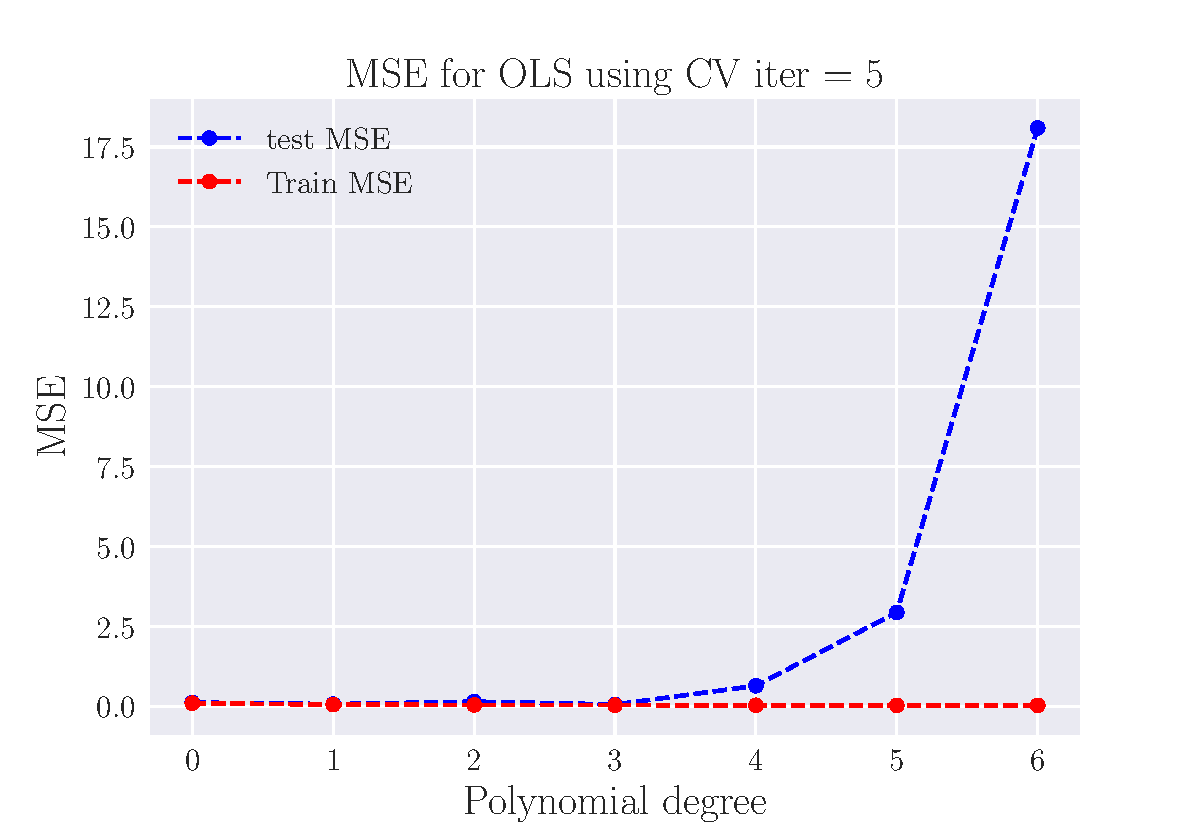
\includegraphics[width=\linewidth]{MSE_OLS_n30_eps02_pol6_CV_re5.pdf}
	\endminipage\hfill
	\minipage{0.49\textwidth}
	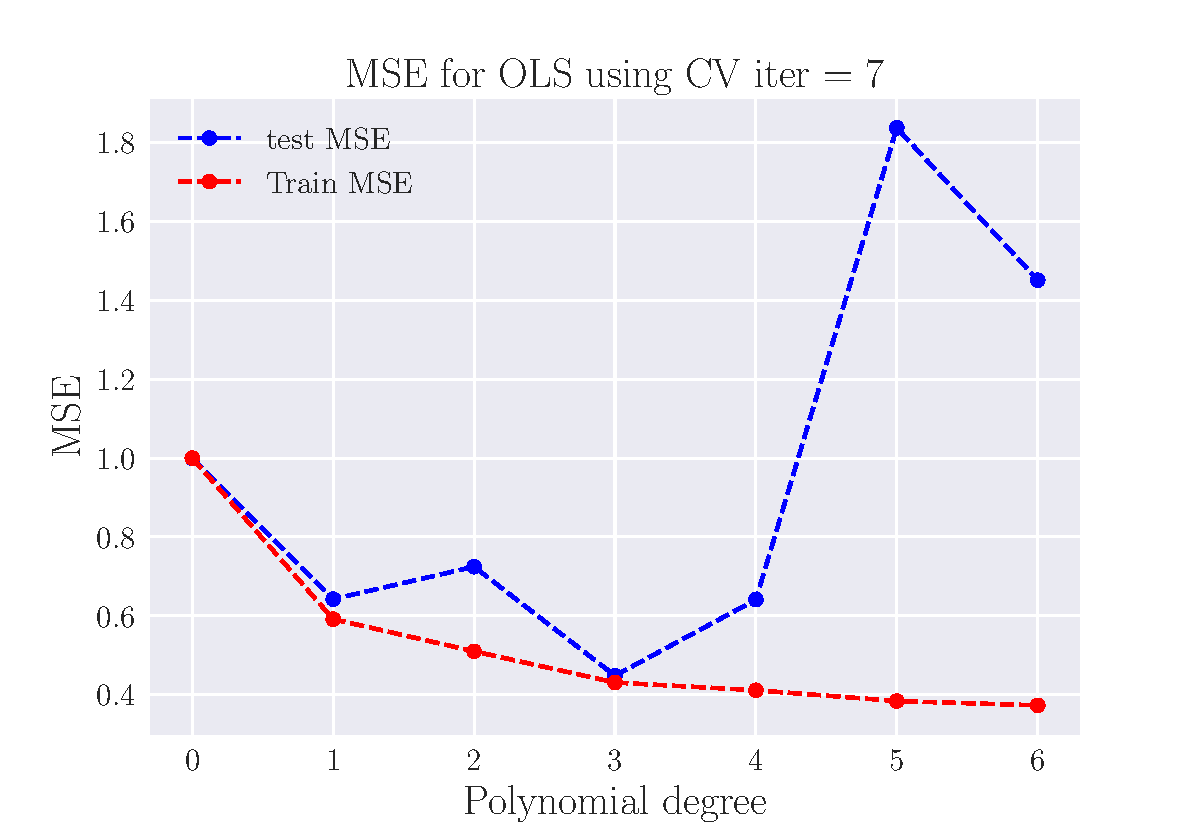
\includegraphics[width=\linewidth]{MSE_OLS_n30_eps02_pol6_CV_re7.pdf}
	\endminipage\hfill
	\minipage{0.49\textwidth}
	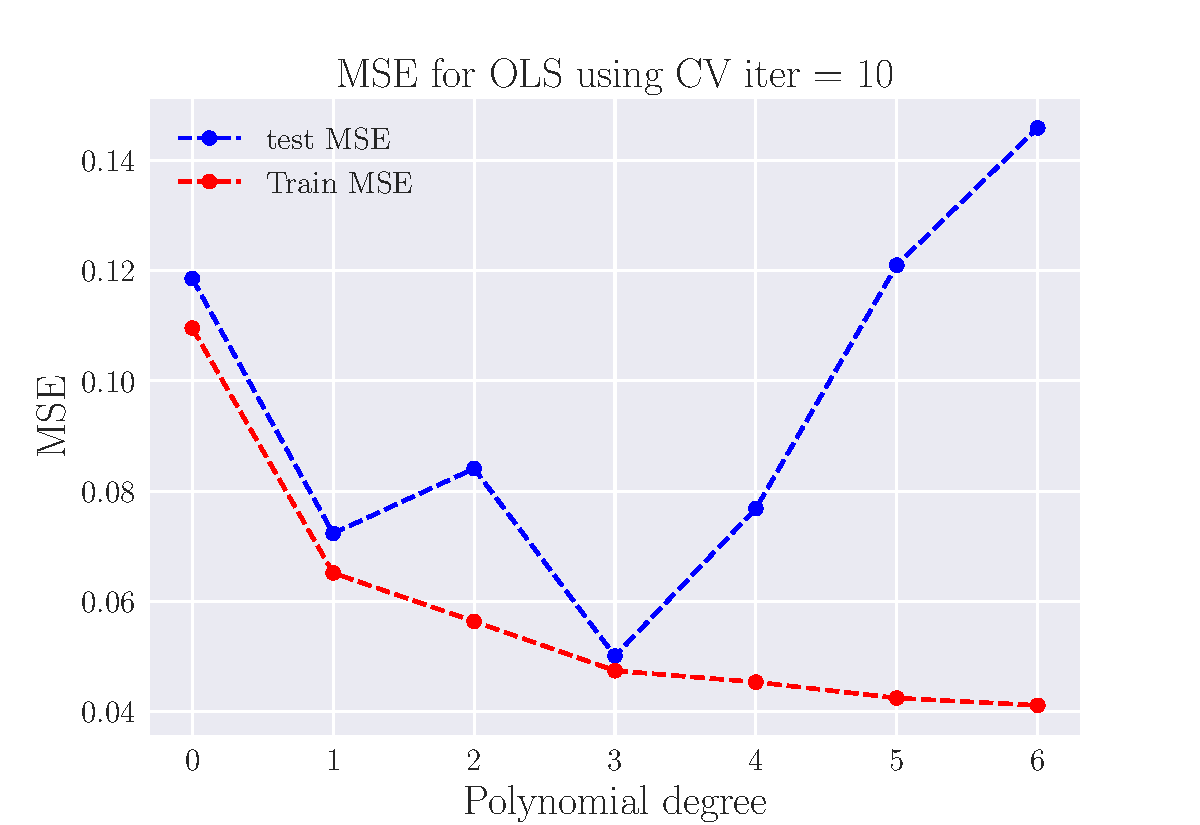
\includegraphics[width=\linewidth]{MSE_OLS_n30_eps02_pol6_CV_re10.pdf}
	\endminipage\hfill
	\minipage{0.49\textwidth}
	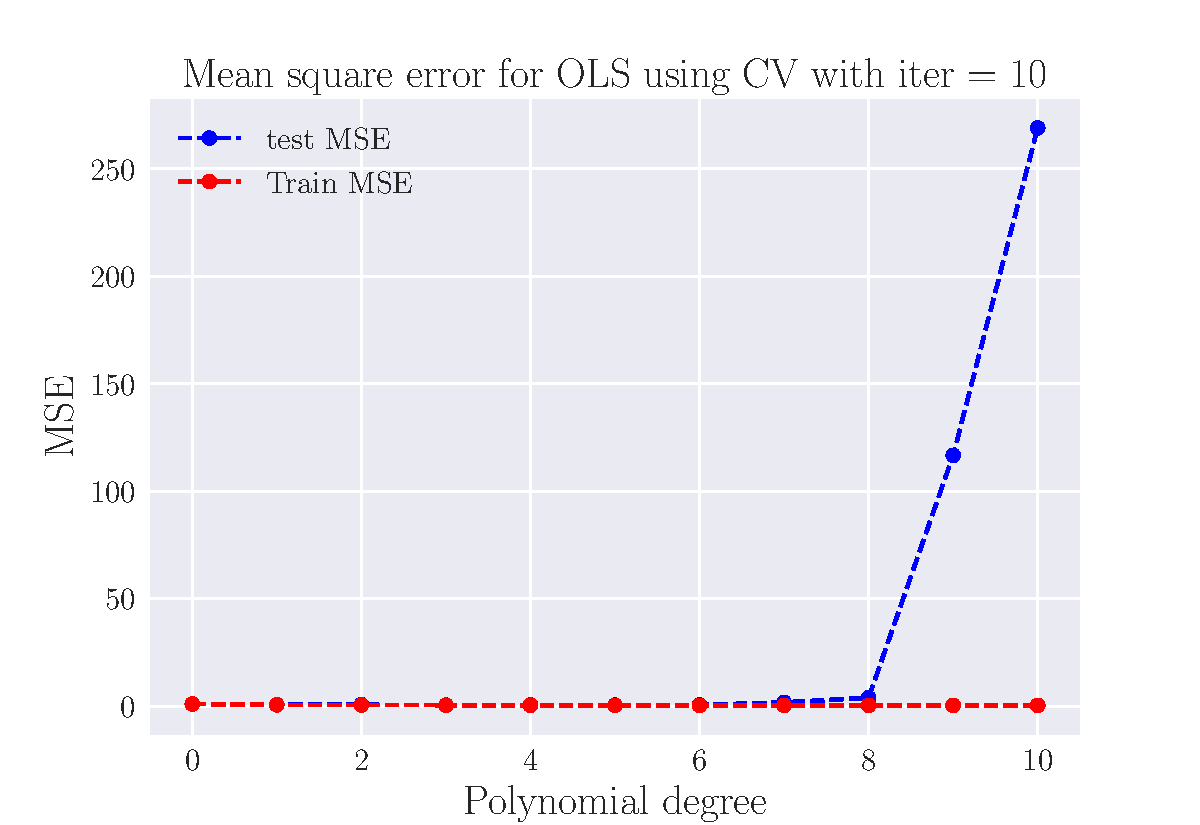
\includegraphics[width=\linewidth]{MSE_OLS_n30_eps02_pol10_CV_re10.pdf}
	\endminipage
	\caption{Here we have plotted the MSE when performing cross-validation as the resampling technique. On the $x$-axis we have polynomial degree, and MSE on the $y$-axis. The top left, right and bottom left figures are with $k=[5, 7, 10]$ iterations respectively. The bottom left plot is to illustrate the diverging MSE for higher polynomial degree, which we see irregardless of iteration-number.} \label{fig:CV_OLS}
\end{figure}

When bootstrapping we saw overfitting at around $p=6$. Looking at the plots in figure \ref{fig:CV_OLS} there seems to be consistent overfitting after around $p=3$. In the bottom right plot we have plotted for higher polynomials to illustrate that this error does not decrease for higher $p$. This diverging behaviour takes place regardless of the number of resampling iterations. We see no obvious reason that the overfitting should start sooner compared to bootstrapping, and thus ground it in random fluctuations. We have consistently seen large variations in results based on number of resampling, and the random seed used when studying the model predictions. The lowest error we get using our standard seed is $MSE_{min}=0.0501$, for $p=3, k=10$.

One possible explanation of the MSE difference between the bootstrap method and cross-validation might be that the test set we used for bootstrap resampling happened to be a favorable one, with fewer points generated with high values of $\epsilon$. Another important aspect is that we averaged a total of $90$ simulations for the bootstrap method, compared to averaging a maximum of $k=10$ resamplings with cross-validation. The mean MSE of the cross-validation method is thus more affected by a bad fit than the mean MSE of the bootstrap method. A further analysis of the resampling methods should therefore include additional simulations where different seed values are studied. This would help us understand the deviations between bootstrapping and cross-validation better, allowing us to conclude whether one of the methods are more suitable. Additionally, it would enable us to estimate whether certain features in our results are a consequence of the specific randomness in the data set.


\section*{Exercise 4: Ridge Regression on the Franke function with resampling}
In some cases, it might happen that the matrix $\mathbf{X}^T\mathbf{X}$ is singular, such that it is non-invertible. This is the case if some of the independent variables are highly correlated. Then OLS will not work, since we invert the matrix in equation \eqref{eq:OLS_beta}. However, by adding a parameter $\lambda$ to the diagonal, the matrix is no longer singular. This is called Ridge regression. The cost-function, $C(X,\bm{\beta})$, and the corresponding optimal parameters, $\boldsymbol{\hat\beta}$, are then given by

\begin{align*}
	C(X,\boldsymbol\beta) &= \frac{1}{n} \left[ \left(\mathbf{y}-\mathbf{X}\boldsymbol\beta\right)^T \left(\mathbf{y}-\mathbf{X}\boldsymbol\beta\right) + \lambda\boldsymbol\beta^T\boldsymbol\beta \right]
	\\
	\boldsymbol{\hat{\beta}} &= (\mathbf{X}^T\mathbf{X}+\lambda \mathbf{I})\mathbf{X}^T\vc{z},
\end{align*}

where $\mathbf{I}$ is  the identity matrix. The parameter $\lambda$ can take any value, so finding the optimal is paramount. This is done by performing regression analyses for many different values of $\lambda$ and choosing the one giving the best results. Note that when $\lambda=0$, the expression becomes that of OLS. The following relation between the Ridge-parameters and the OLS-parameters can be show to be true:
\begin{equation}\label{eq:beta_ridge_ols}
	\hat{\beta}^{Ridge} = (1 + \lambda)^{-1}\hat{\beta}^{OLS}
\end{equation}

Before we look at specific values of $\lambda$ or polynomial degrees, we make a heatmap of the MSE for several values of both, since the optimal $\lambda$-values depends on the polynomial degree in question. As equation \eqref{eq:beta_ridge_ols} shows, the $\hat{\beta}^{Ridge}$ parameters go to $0$ for large values of $\lambda$. Higher $\lambda$ values will therefore suppress the $\hat{\beta}^{OLS}$ parameters, so we expect the best $\lambda$-value to be quite small, since the OLS regression resulted in relatively low MSE values, indicating a good fit. In figure \ref{fig:Ridge-boot_heatmap}, we have chosen values between $10^{-6}$ and $10^0$. The polynomial degree run from $1$ to $15$. The 0-polynomial is excluded as it would be extreme underfitting, giving high errors and reduces details related the magnitude of other error values.

\begin{figure}[h]
	\begin{center}
		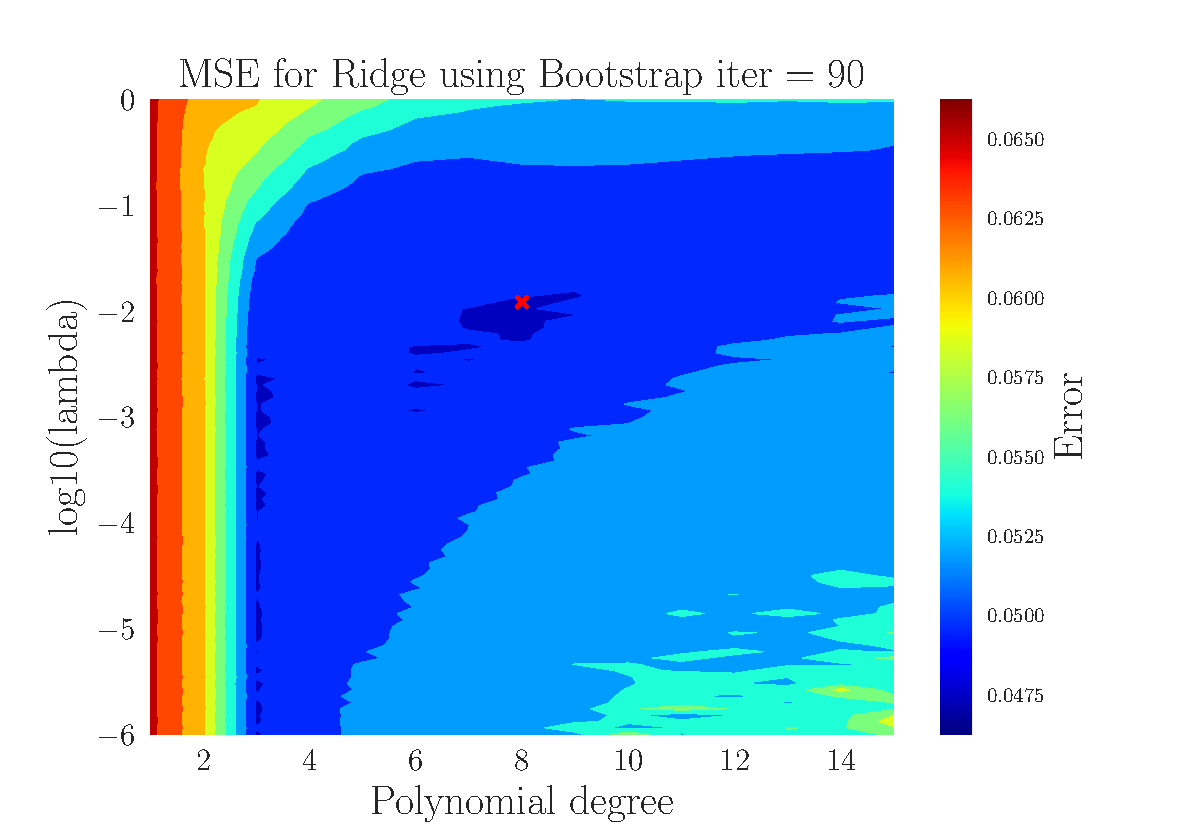
\includegraphics[width=0.8\linewidth]{Contour_PL_Ridge_Bootstrap90_n30_eps0.2_p1_15_lmb0_m6.pdf}
	\end{center}
	\caption{Test MSE using Ridge and bootstrapping, as function of polynomial degree and $\lambda$. The minimum value is $MSE=0.0472$ at $p=8$ and $log10(\lambda_{min}) = -2.07$, indicated by the red cross.}
	\label{fig:Ridge-boot_heatmap}
\end{figure}

There are several regions to note in figure \ref{fig:Ridge-boot_heatmap}. Firstly, for low polynomial degrees, all $\lambda$ values gives high MSE values. This is underfitting. Next, the MSE is also high for high polynomial degrees when the $\lambda$ values are low. This is a region of overfitting. It does not extend up to higher $\lambda$s. This is probably because the estimators related to the higher order polynomials are being supressed, as per \eqref{eq:beta_ridge_ols}, preventing them from dominating the overall prediction. Lastly, the MSE is smallest in a region around $p=8$ and $\lambda=10^{-2.07}$, which is a higher polynomial degree than we got from our OLS analyses. This point yields $MSE_\text{min}=0.0471$, which is a lower value than obtained when bootstrapping with OLS, although marginally. With OLS we also got that $p=3$ yielded the lowest test MSE overall when bootstrapping, and in figure \ref{fig:Ridge-boot_heatmap} we see a thin vertical region for $p=3$ where the MSE is lower compared to neighbouring polynomial degrees. As a final note, we see that the narrow regions with lower MSE values are found near $p=6$ as well, with certain regions covering $p=7$ as well.

We now want to do the same analysis, using cross-validation instead of bootstrapping. We make a new heatmap, in the same $\lambda$-range as in figure \ref{fig:Ridge-boot_heatmap}, but limit ourselves to lower polynomials, as the MSE values for CV using OLS were quite large for high polynomial degrees. A plot up to $p=10$ was generated, but the high MSE values for larger values of $p$ caused the remaining MSE values to appear identical, so we have chosen to not include it.

<<<<<<< HEAD
Figure \ref{fig:Ridge_CV_heatmap} is similar to figure \ref{fig:Ridge-boot_heatmap}, the corresponding plot for bootstrapping, in that very low polynomial orders and high $\lambda$ values, as well as high polynomial degrees with low $\lambda$ values, gives a high MSE. The lowest errors are found within a region around $\lambda\in[10^{-1},\,10^{-3}]$ for $p>3$. The lowest MSE value is $MSE_\text{min}=0.0493$, for $p=3,\, \lambda=10^{-2.24}$. Our study of resampling methods with ridge regression thus yielded similar result as it did for OLS, where cross validation caused a distinct increas in the MSE for $p>3$, while it remained low for bootstrapping until we reached $p>8$.
=======
Figure \ref{fig:Ridge_CV_heatmap} is similar to figure \ref{fig:Ridge-boot_heatmap}, the corresponding plot for bootstrapping, in that very low polynomial orders and high $\lambda$ values, as well as high polynomial degrees with low $\lambda$ values, gives a high MSE. The lowest errors are found within a region around $\lambda\in[10^{-1},\,10^{-3}]$ for $p>3$. The lowest MSE value is $MSE_\text{min}=0.0493$, for $p=3,\, \lambda=10^{-2.24}$.
>>>>>>> 36eb51052d5a528a58678a456f21a0858b9beb66

\begin{figure}[h]
	\begin{center}
		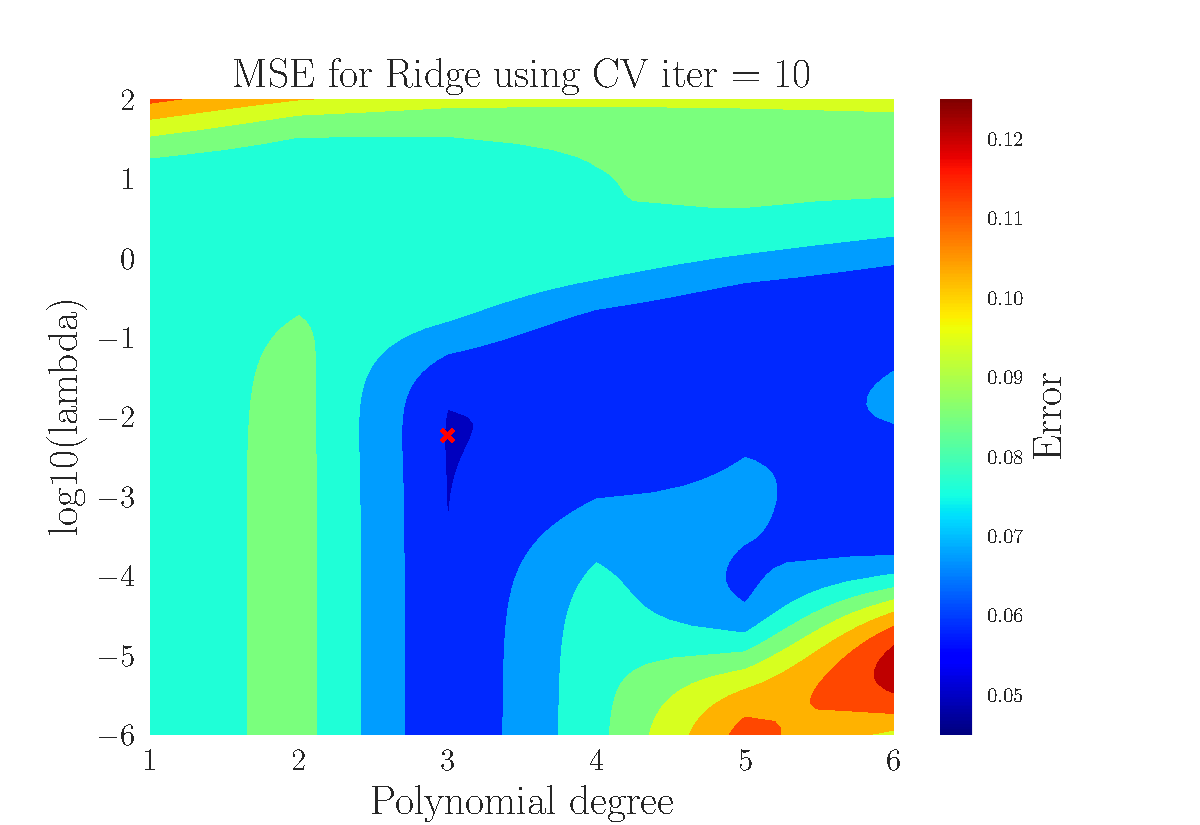
\includegraphics[width=0.8\linewidth]{Contour_PL_Ridge_CV10_n30_eps0.2_p1_6_lmb2_m6.pdf}
	\end{center}
	\caption{MSE using Ridge with cross-validation, k=10, as function of $\lambda$ and polynomial degree. The minimum value is $MSE=0.0493$ at $p=3$ and $log10(\lambda)=-2.24$)}
	\label{fig:Ridge_CV_heatmap}
\end{figure}

Since we were able to get a slightly better $MSE_\text{min}$ with ridge, as compared to OLS, it indicates that Ridge-regression is somewhat better than normal OLS, but not by much. The best results when using Ridge did arise from very small $\lambda$ values, making the method virtually similar to OLS. Another advantage of the ridge regression was that the $\lambda$ parameter provided more options for higher order polynomials, making our model less sensitive to one specific choice. Before making any conclusions, we will perform a bias-variance trade-off analysis for ridge regression.

To study the regression method further, we now want to study the bias-variance trade-off using Ridge. Using high $\lambda$, Ridge should suppress the estimators, giving very low variance, even for high polynomial degrees. The bias should for the same reason be high, as this would be akin to underfitting. For low $\lambda$, the variance should be much higher, as this is similar to OLS.  Using 3 values for $\lambda$, figure \ref{fig:Ridge_boot_BVT} shows the bias, variance and error for polynomials between $p=0$ and $p=20$. For $\lambda=100$, Ridge suppresses the estimators.   the bias quickly converges to a value, and the variance never increases.

\begin{figure}[h]
	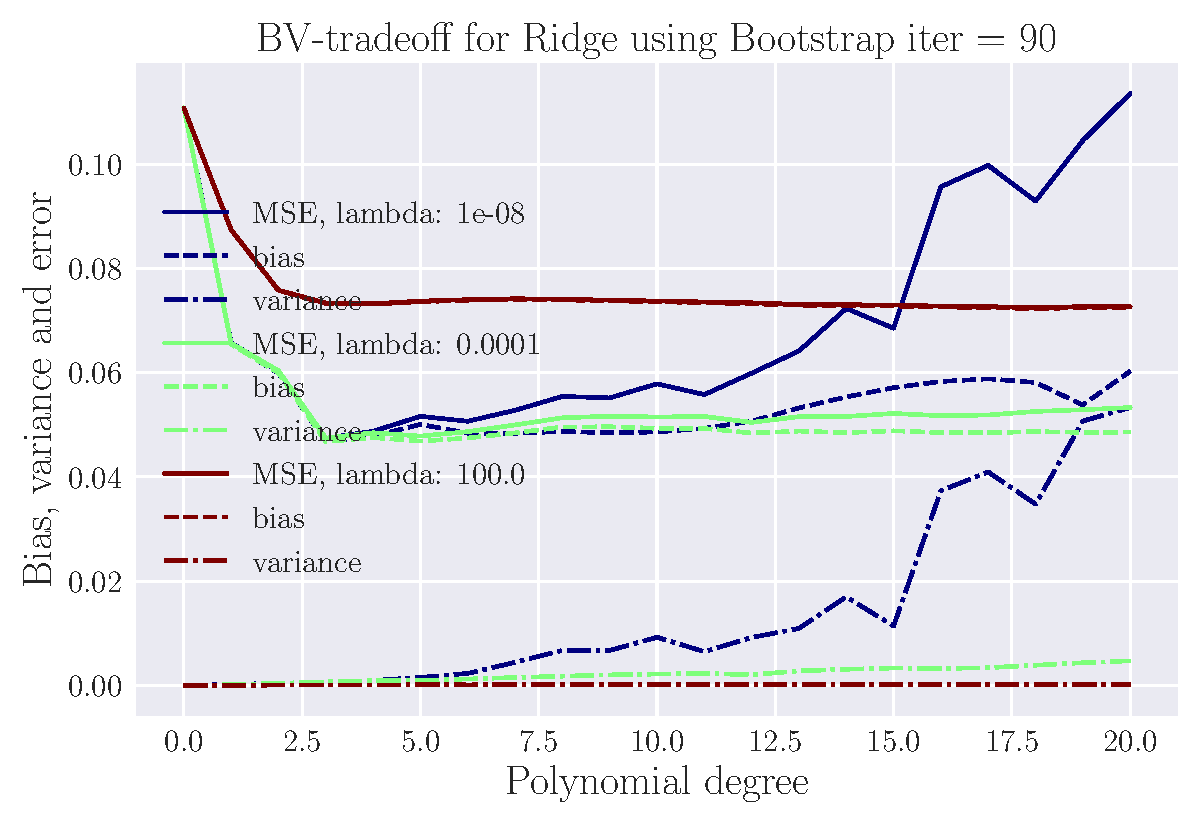
\includegraphics[width=\linewidth]{LBVT_Ridge_Bootstrap_n30_eps0_2_p20_lmbm8_2.pdf}
	\caption{MSE, bias and variance using Ridge and bootstrapping, for different $\lambda$s.}
	\label{fig:Ridge_boot_BVT}This is the lowest error of any method so far in this paper.
\end{figure}


%\begin{figure}[H]
%	\minipage{0.49\textwidth}
%	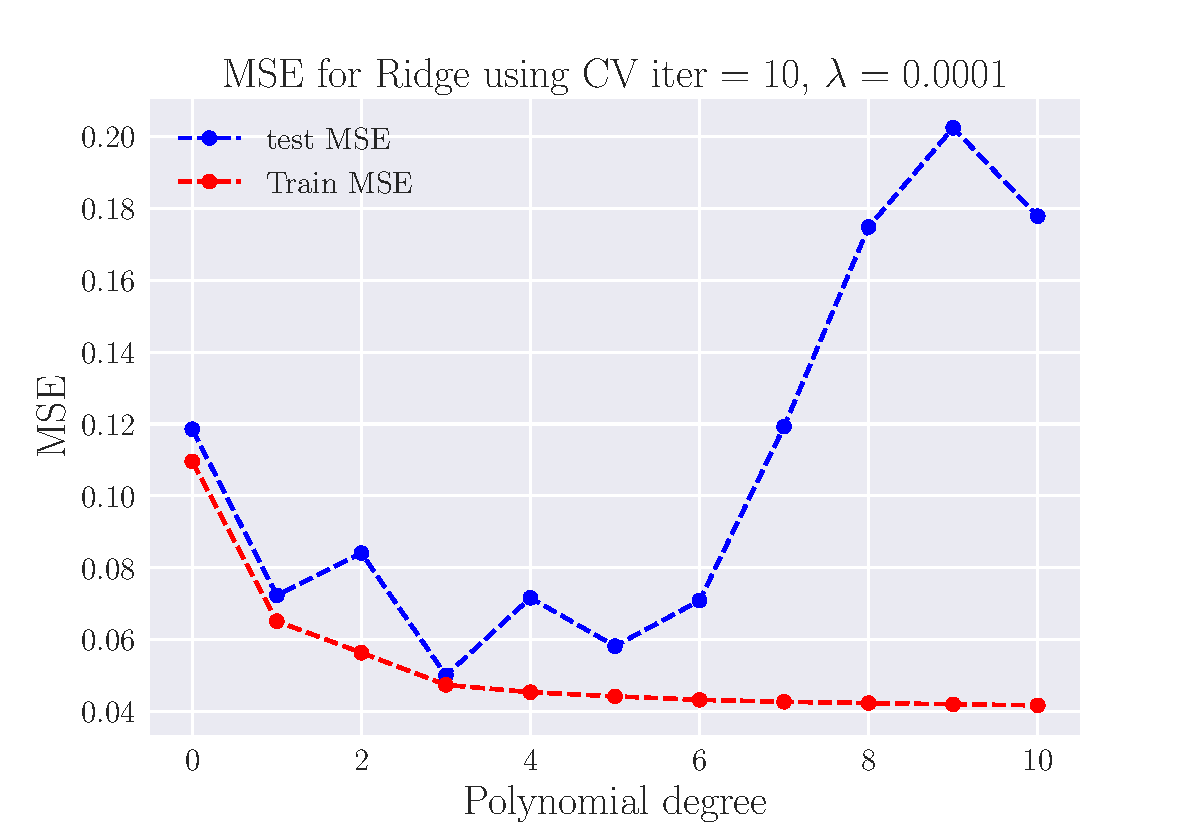
\includegraphics[width=\linewidth]{MSE_Ridge_n30_eps02_pol10_CV_re10_lam_0_0001.pdf}
%	\endminipage\hfill
%	\minipage{0.49\textwidth}
%	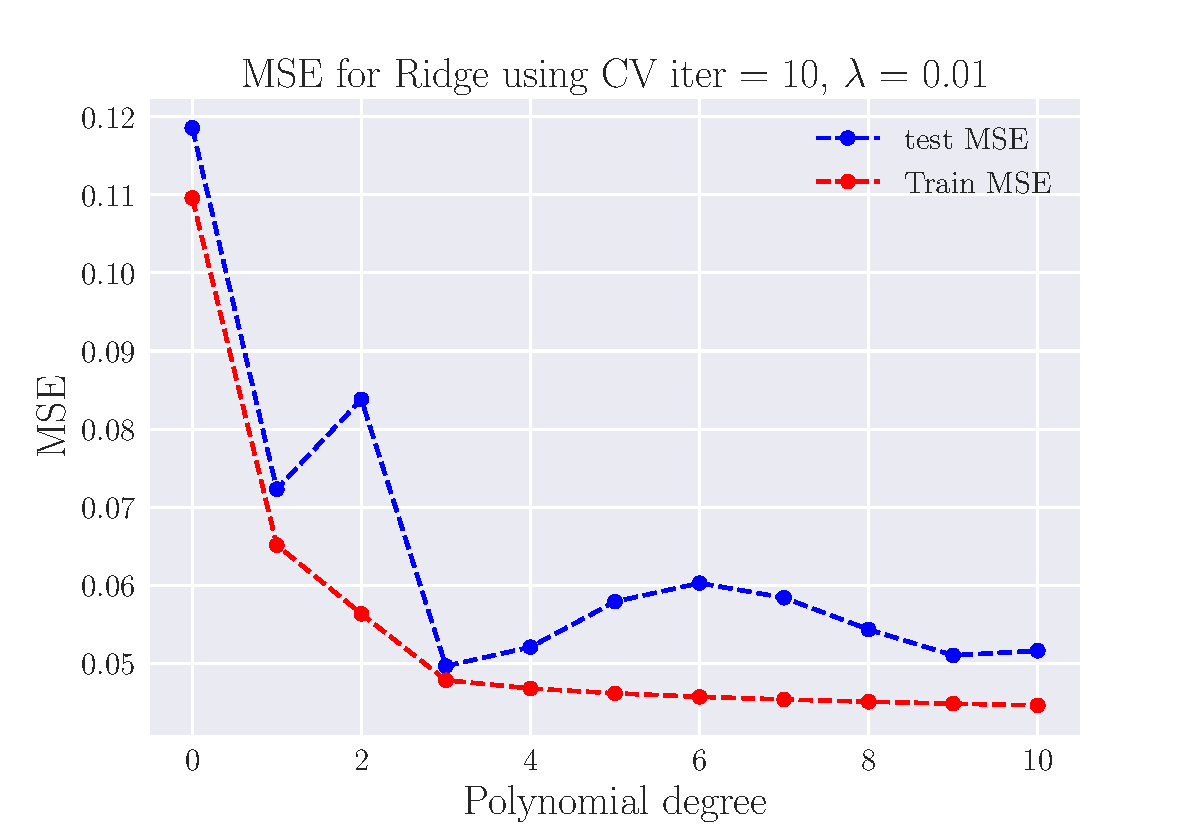
\includegraphics[width=\linewidth]{MSE_Ridge_n30_eps02_pol10_CV_re10_lam_0_01.pdf}
%	\endminipage\hfill
%	\minipage{0.49\textwidth}
%	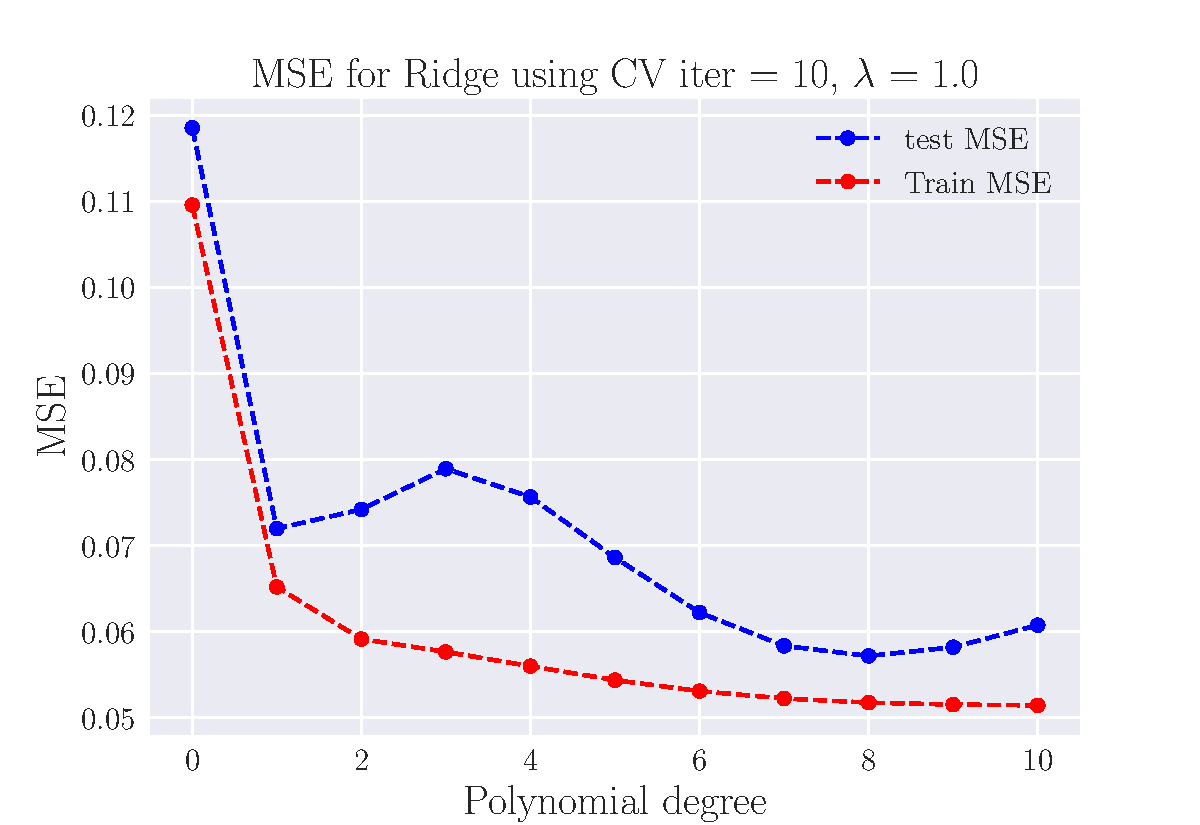
\includegraphics[width=\linewidth]{MSE_Ridge_n30_eps02_pol10_CV_re10_lam_1_0.pdf}
%	\endminipage\hfill
%	\minipage{0.49\textwidth}
%	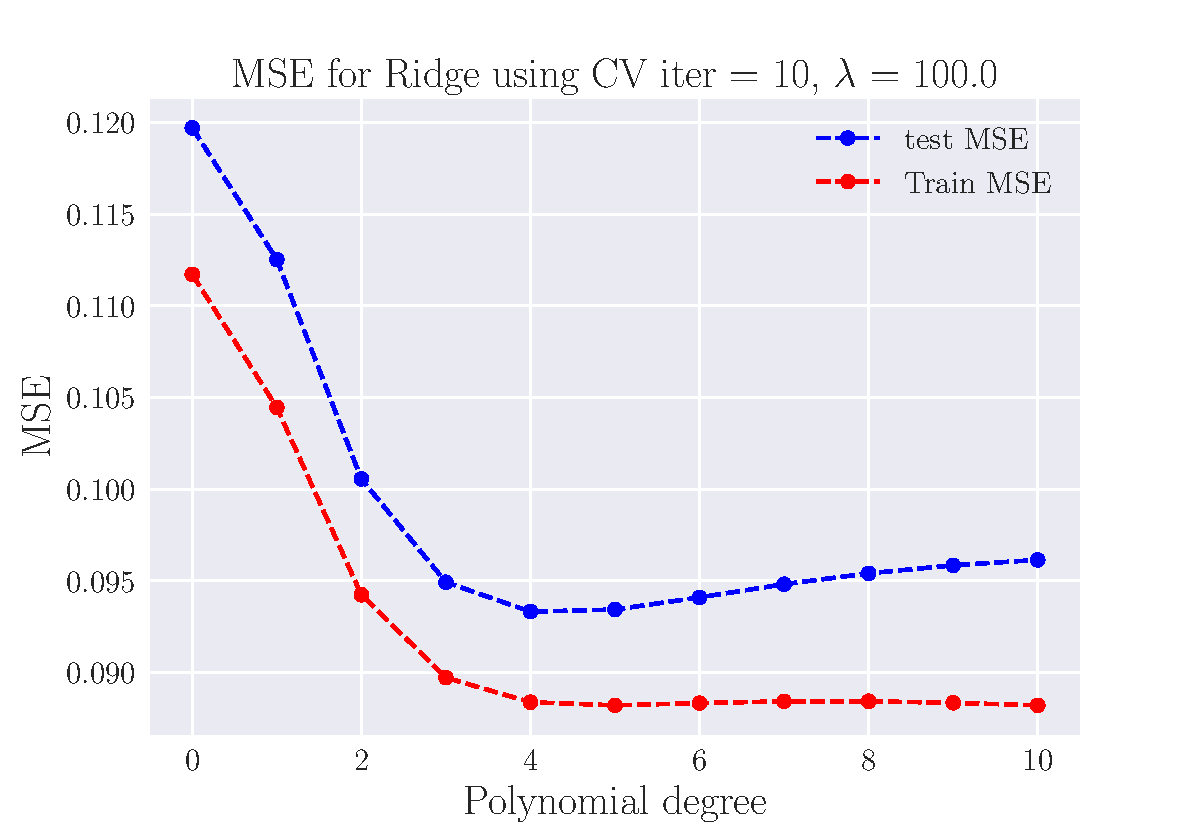
\includegraphics[width=\linewidth]{MSE_Ridge_n30_eps02_pol10_CV_re10_lam_100_0.pdf}
%	\endminipage
%	\caption{MSE using Ridgeregression and cross-validation, as function of complexity, for different values of $\lambda$.} \label{fig:Ridge_CV_PM}
%\end{figure}


\section*{Exercise 5: Lasso regression on the Franke function with resampling}

A third regression method is Lasso. This has the following cost-function:
\begin{equation*}
	C(\mathbf{X}, \boldsymbol{\beta}) = \frac{1}{n}\left[\left(\mathbf{y}-\mathbf{X}\boldsymbol\beta \right)^T \left(\mathbf{y}-\mathbf{X}\boldsymbol\beta \right)+\lambda ||\boldsymbol{\beta}||_1 \right].
\end{equation*}
The optimal parameters do not have a nice, simple expression, due to the L1-norm. For this reason we do not implement the method ourselves in the code, rather calling the function from a package (scikit-learn).  The main difference between Ridge and Lasso is that while Ridge suppresses the estimators for as function of $\lambda$, Lasso sets the estimators to 0 for some $\lambda$. Again, as is the case for Ridge, for very low $\lambda$, this should be the same as OLS.

In figure \ref{fig:Lasso_boot_heatmap}, we choose $\lambda$ in the range $10^{-6}$ to $10^{-1}$. For higher values, the error is exactly the same everywhere, as we should expect from Lasso. The polynomial degree range from 1 to 10. Lasso is extremely slow, so higher polynomial degrees and lower $\lambda$ is not viable to get results for in reasonable time. We see in the figure that the error is high for higher $\lambda$, and decrease along with it. We clearly see the underfit for low polynomial degrees, but have not reached the overfit for higher, as we saw in figures \ref{fig:Ridge-boot_heatmap} and \ref{fig:Ridge_CV_heatmap} for Ridge. We do however see a dip in the errors, along $lambda=10^{-5}$. This indicates that Lasso might give better results than OLS, as there is a benefit in not using as low as possible $\lambda$. The lowest error we get is $MSE_{min}=0.0473$ for $p=7$ and $\lambda=10^{-5.0}$. 

\begin{figure}[h]
	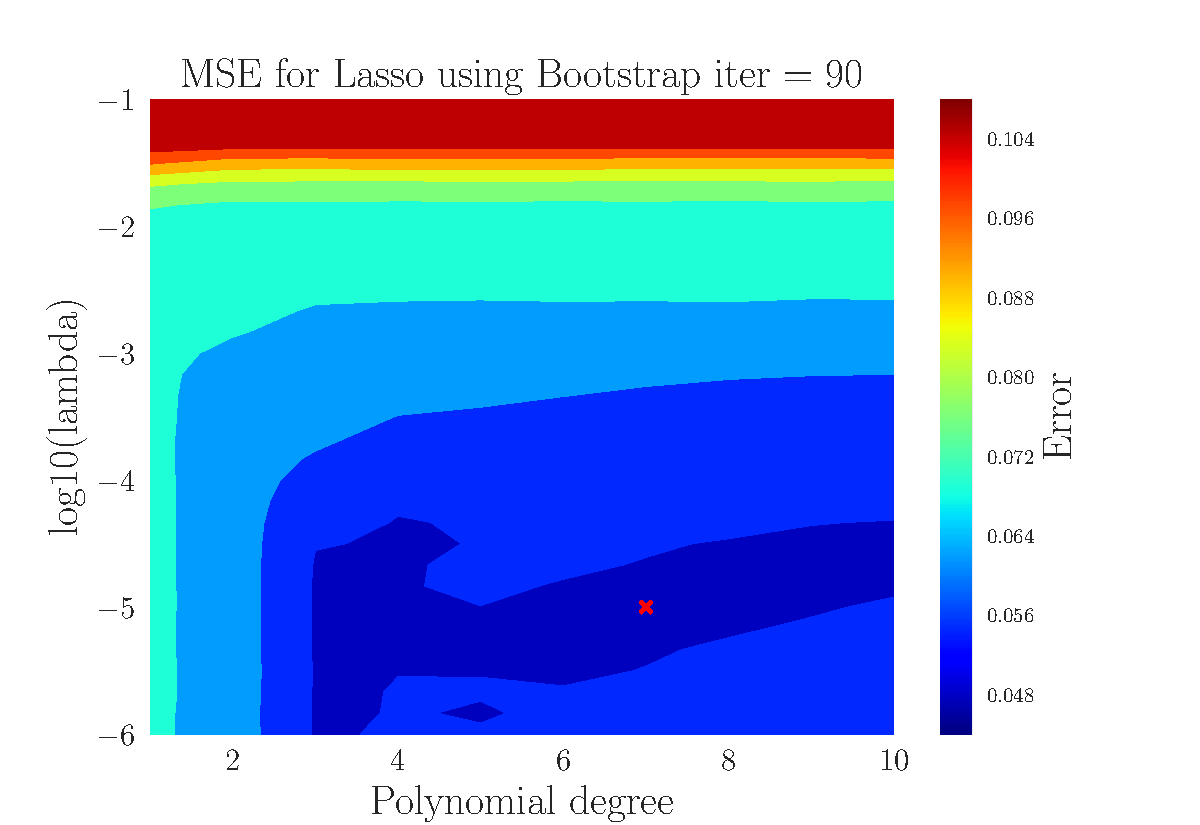
\includegraphics[width=\linewidth]{Contour_PL_Lasso_Bootstrap90_n30_eps0.2_p1_10_lmbm1_m6.pdf}
	\caption{MSE using Lasso with bootstrapping, as function of $\lambda$ and polynomial degrees. The lowest error is $MSE_{min}=0.0473$, for $p=7$ and $\lambda = 10^{-5.0}$.}
	\label{fig:Lasso_boot_heatmap}
\end{figure}

MÅ OGSÅ GJØRE BVT. jeg driver å lager plottet nå

As we did for Ridge-regression, we want also to run Lasso with cross-validation. At this point, our code gives us some very weird results. We should get that Lasso gives low errors for low $\lambda$, just as with OLS, increasing till a point where it becomes a straight line. This is what we got using bootstrapping. However, using CV we do not get this, see figure \ref{fig:Lasso_CV_heatmaps}. The error is high for low $\lambda$, and decrease as $\lambda$ increase, leveling out at some point. The upper plot shows the $log10$ of the error, so the uniform colour indicates that the error is the same everywhere in the upper region. The lower plot almost looks like it is the inverse of figure \ref{fig:Ridge_CV_heatmap}, the corresponding one for Ridge. This makes it look like we are simply plotting the results the wrong way. Having indulged this idea, messing with the code in attempts at reversing it, this has been ruled out. Had there been such a bug somewhere it should have revealed itself in our earlier results. It is the same functions that are being called, in different combinations. Only the combination Lasso with cross-validation gives these results. The analysis and plotting is exactly the same for all the heatmap-plots. What makes this problem even weirder and hard to resolve is that we do not get this with the terrain data. In the next section we will thus present Lasso-CV-results, which we have confidence in to be correct. We will get back to this then, but we are choosing a smaller region in the entire data to analyse. To further exacerbate the weirdness of the bug, by choosing a region of same size right next to the original in the same datafile, we again get the same wrong results as here with the Franke function. Intense staring at the code by multiple people outside our group has resulted in nothing further than several "Huh, that's weird. It shouldn't do that."


\begin{figure}[h]
	\minipage{0.80\textwidth}
	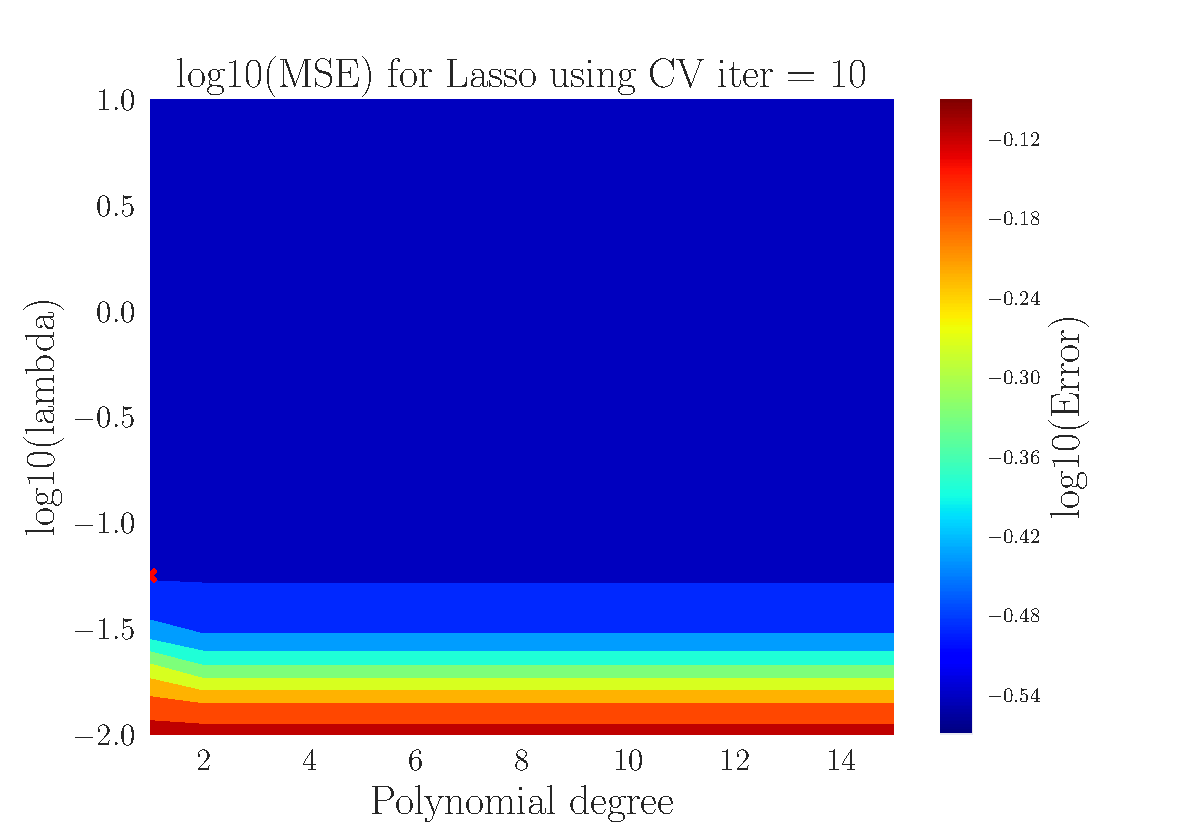
\includegraphics[width=\linewidth]{Contour_PL_Lasso_CV10_n30_eps0.2_p1_15_lmb1_m2.pdf}
	\endminipage\hfill
	\minipage{0.80\textwidth}
	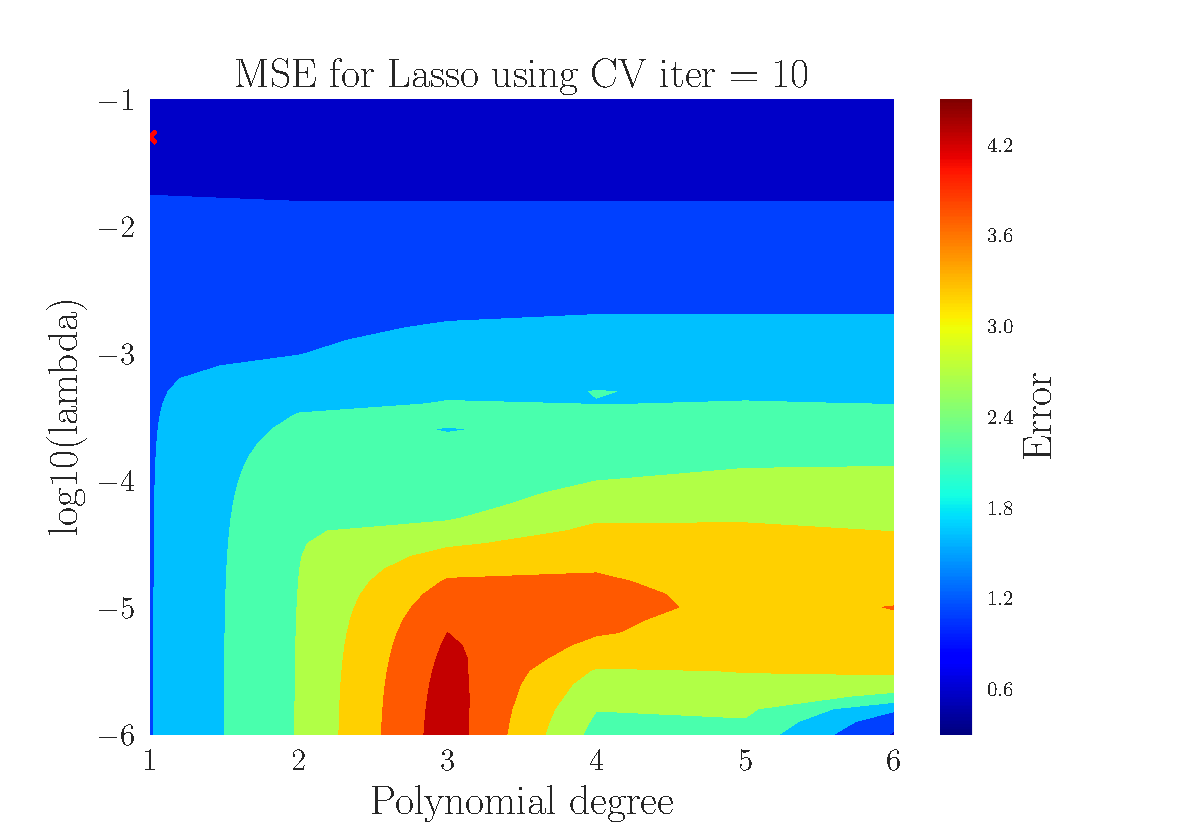
\includegraphics[width=\linewidth]{Contour_PL_Lasso_CV10_n30_eps0.2_p1_6_lmbm1_m6.pdf}
	\endminipage
	\caption{MSE using Lasso and cross-validation, for a wide range of $\lambda$ and polynomial degrees. The upper plot is with $log10(MSE)$, while on the bottom is just the $MSE$.}
	\label{fig:Lasso_CV_heatmaps}
\end{figure}

\clearpage
\section*{Exercise 6: Analysis of real data}
Having used our data analysis methods to study the Franke function we will now move on to study data from the real world. We will consider Norwegian terrain data from here\footnote{\href{https://github.com/CompPhysics/MachineLearning/tree/master/doc/Projects/2021/Project1/DataFiles}{https://github.com/CompPhysics/MachineLearning/tree/master/doc/Projects/2021/Project1/DataFiles}}. Because the datasets are large, we will only consider one small part of \texttt{SRTM\_data\_Norway\_1.tif}, namely $f_{i,j}$ where $i,j\in[50,100]$, i.e. $N=50$ datapoints in each direction. It is useful to consider dimensionless data, thus we divide by the absolute highest/lowest point $z_{i,j} = f_{i,j}/\max{|f_{i,j}|}$, and let $i,j\in[50,100] \rightarrow x,y\in[0,1]$ when plotting. Then we get the data visualized in figure \ref{fig:terrain_raw}.

\begin{figure}[h]
	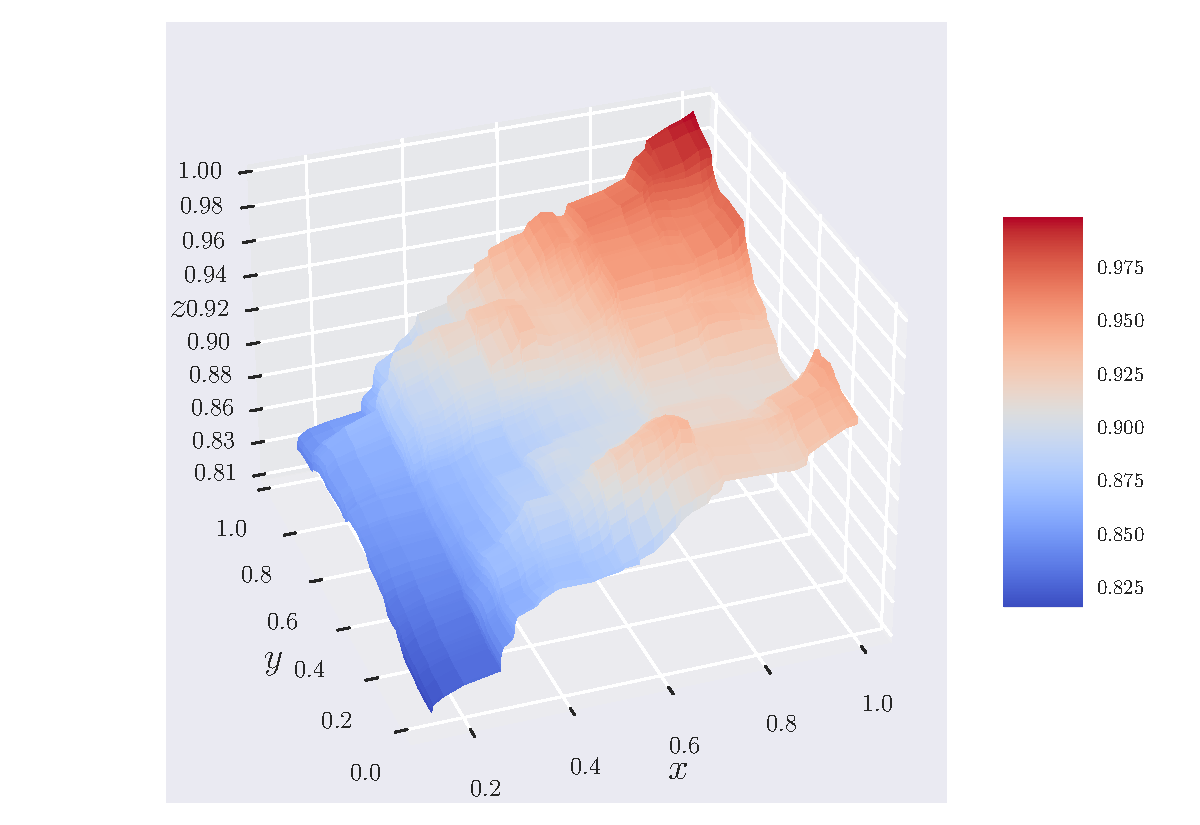
\includegraphics[width=\linewidth]{SRTM_rawdata_n50.pdf}
	\caption{Here we have plotted the terrain data which we will use in this exercise.}
	\label{fig:terrain_raw}
\end{figure}

We will analyze the data using the same methods above. Namely OLS, Ridge- and Lasso-regression. We will implement Bootstrapping and cross validation for them all, and try to evaluate bias and variance. The first three sections (OLS, Ridge and Lasso) will cover each numerical method separately. Then in the last section (Analysis) we will try to conclude which one is best.

\subsection*{OLS}
We begin by studying the MSE using OLS-regression and bootstrapping as the resampling technique. Our results should mirror those we got in exercise 2, where the test MSE decreases in the beginning, and increases when we start overfitting. Choosing $B = 50$ iterations and max polynomial degree $p_\text{max} = 30$ we get the MSE illustrated in figure \ref{fig:terrain_OLS_MSE_bootstrap}. Because of the small variation in MSE we plotted the $\log(\text{MSE})$ along the $y$-axis.

\begin{figure}[h]
  \minipage{0.49\textwidth}
  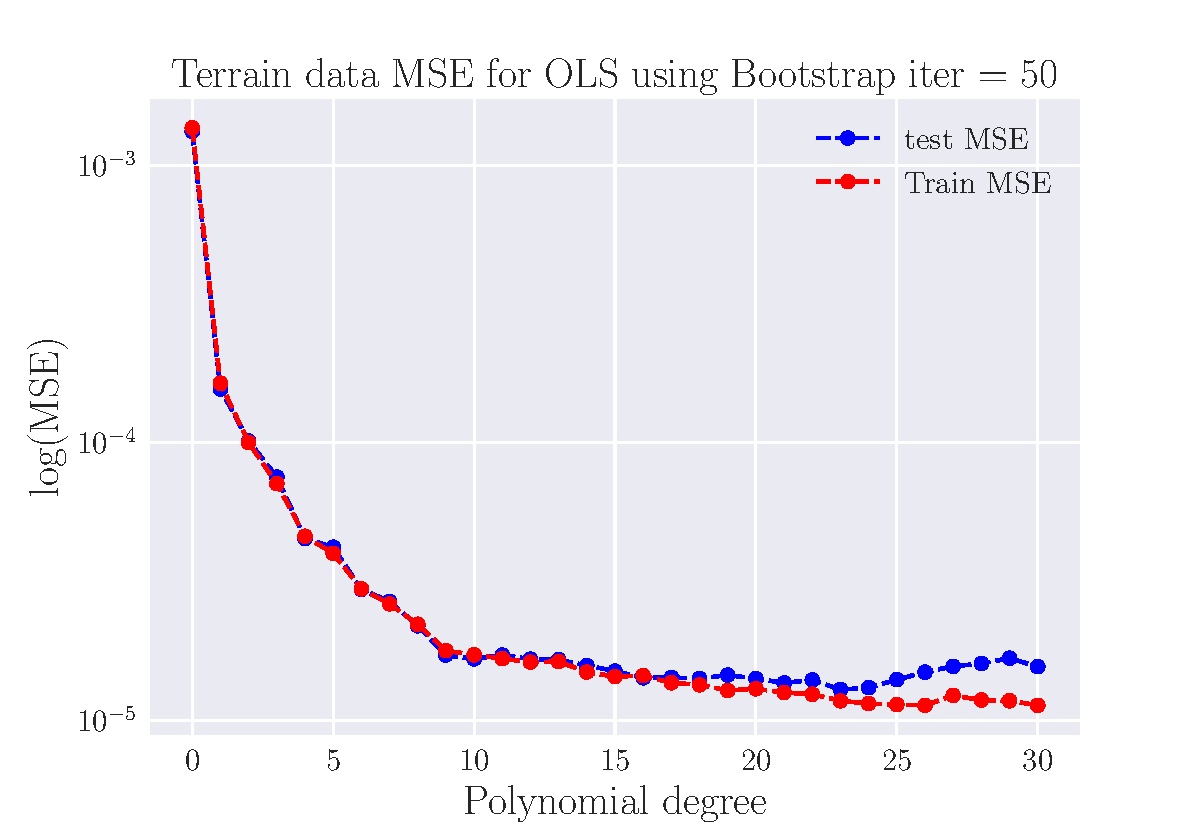
\includegraphics[width=\linewidth]{SRTM_MSE_OLS_n50_pol30_Bootstrap_re50_log.pdf}
  \endminipage\hfill
  \minipage{0.49\textwidth}
  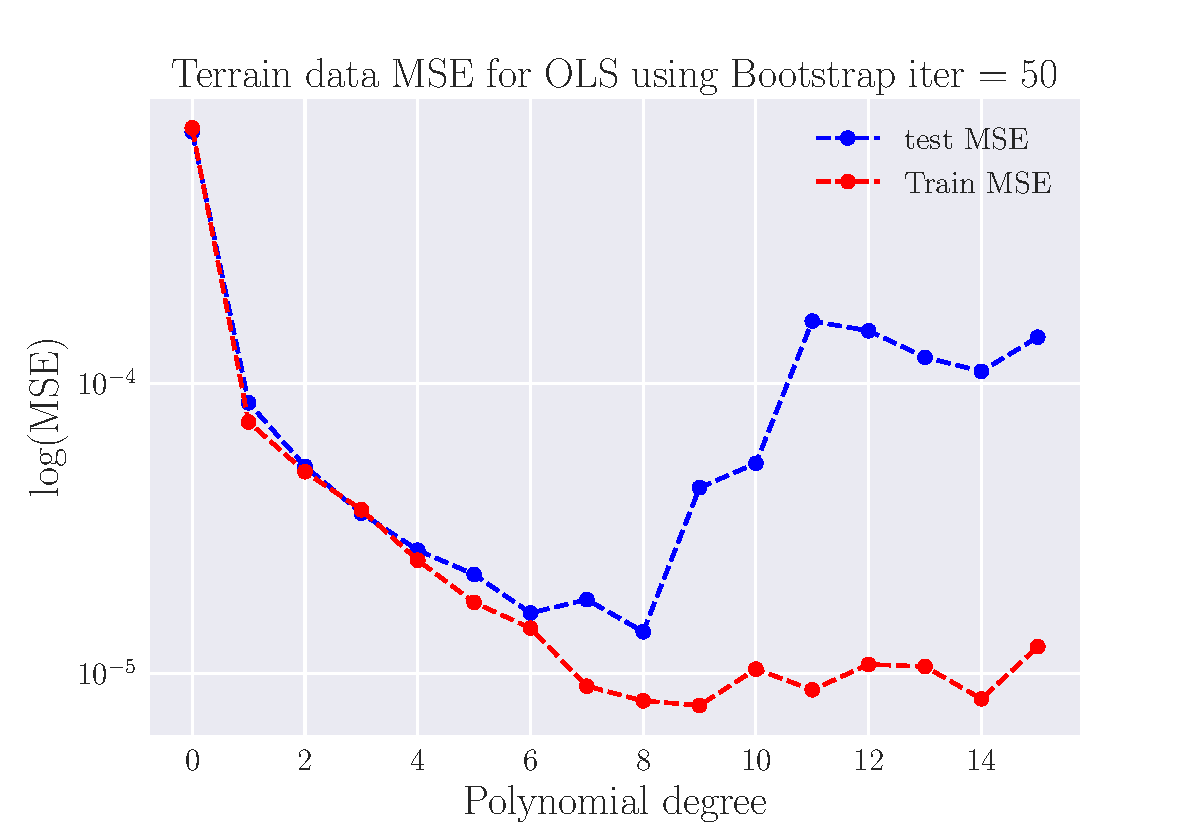
\includegraphics[width=\linewidth]{SRTM_MSE_OLS_n30_pol15_Bootstrap_re50_log.pdf}
  \endminipage
  \caption{Her we have plotted the $\log(\text{MSE})$ as a function of polynomial degree. The left plot is with $(50\cross50)$ grid-points and right with $(30\cross30)$.}
  \label{fig:terrain_OLS_MSE_bootstrap}
\end{figure}
Looking at figure \ref{fig:terrain_OLS_MSE_bootstrap} we see that for $(50\cross50)$ grid-points (left plot), we get a small increase in the MSE after $p = 23$. The actual minimum $\text{MSE} \approx 1.29\cdot10^{-5}$ is at polynomial degree $p = 23$. We assume that overfitting is not evident due to the large number of data points. Therefore we plot for $30\cross30$ grid-points (right figure) and see a much larger increase after $p = 8$. Because of this we conclude that the small overfitting is due to our large number of grid-points.

As a simple sanity check, we plot the result of our fits for different polynomial degrees, which we can compare to the original data from figure \ref{fig:terrain_raw}. To capture the complexity of our data set, we consider four polynomial degrees, using $p\in[10,\,20,\,30,\,50]$, where the first two are shown in the upper left and right panel of figure \ref{fig:terrain_fit}, respectively, while the latter two in the bottom left and right panel of the same figure, respectively.

\begin{figure}[h]
	\minipage{0.49\textwidth}
	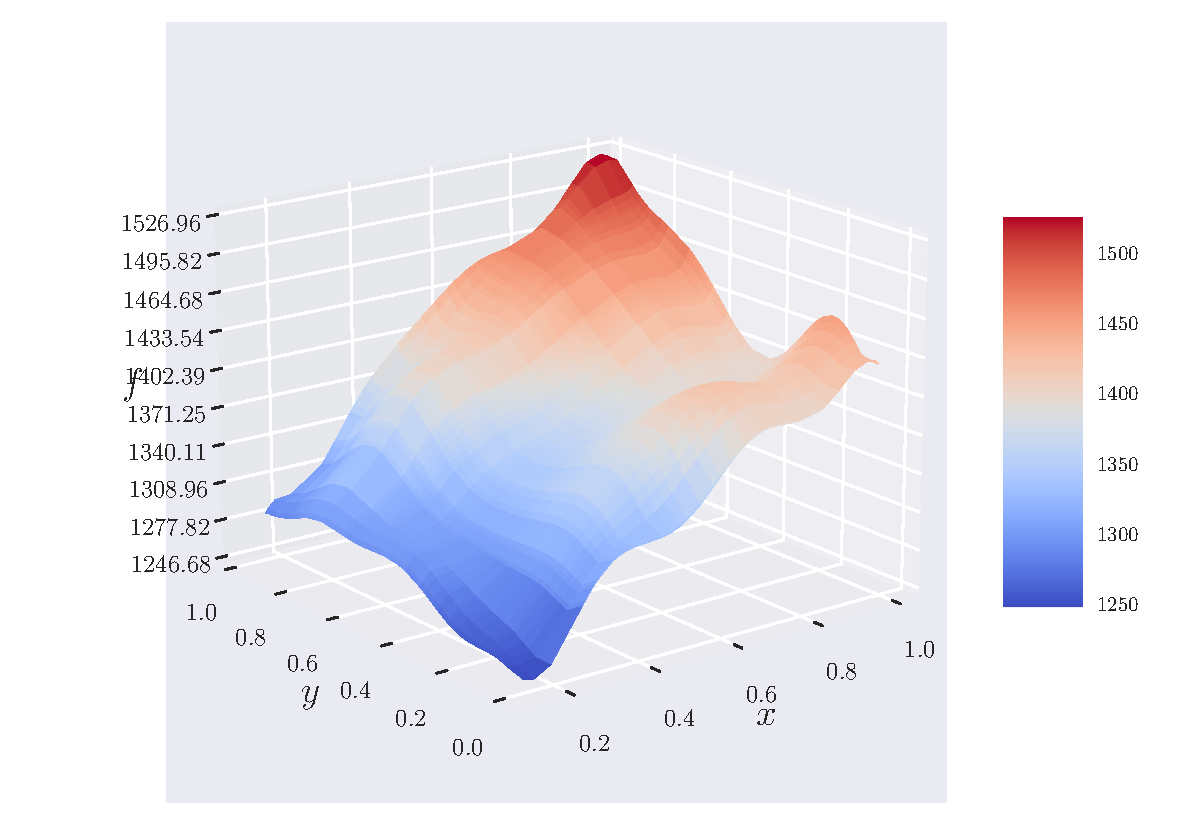
\includegraphics[width=\linewidth]{SRTM_prediction_p10.pdf}
	\endminipage\hfill
	\minipage{0.49\textwidth}
	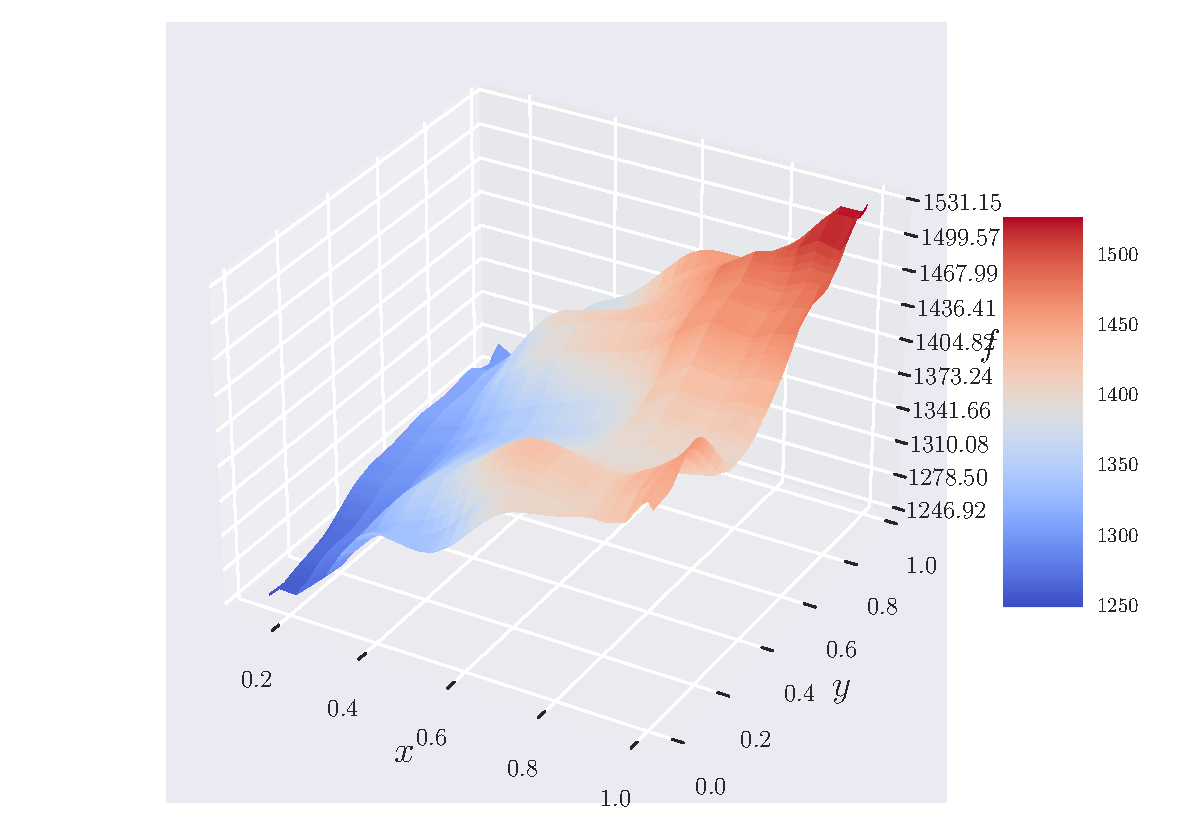
\includegraphics[width=\linewidth]{SRTM_prediction_p20.pdf}
	\endminipage\hfill
  \minipage{0.49\textwidth}
	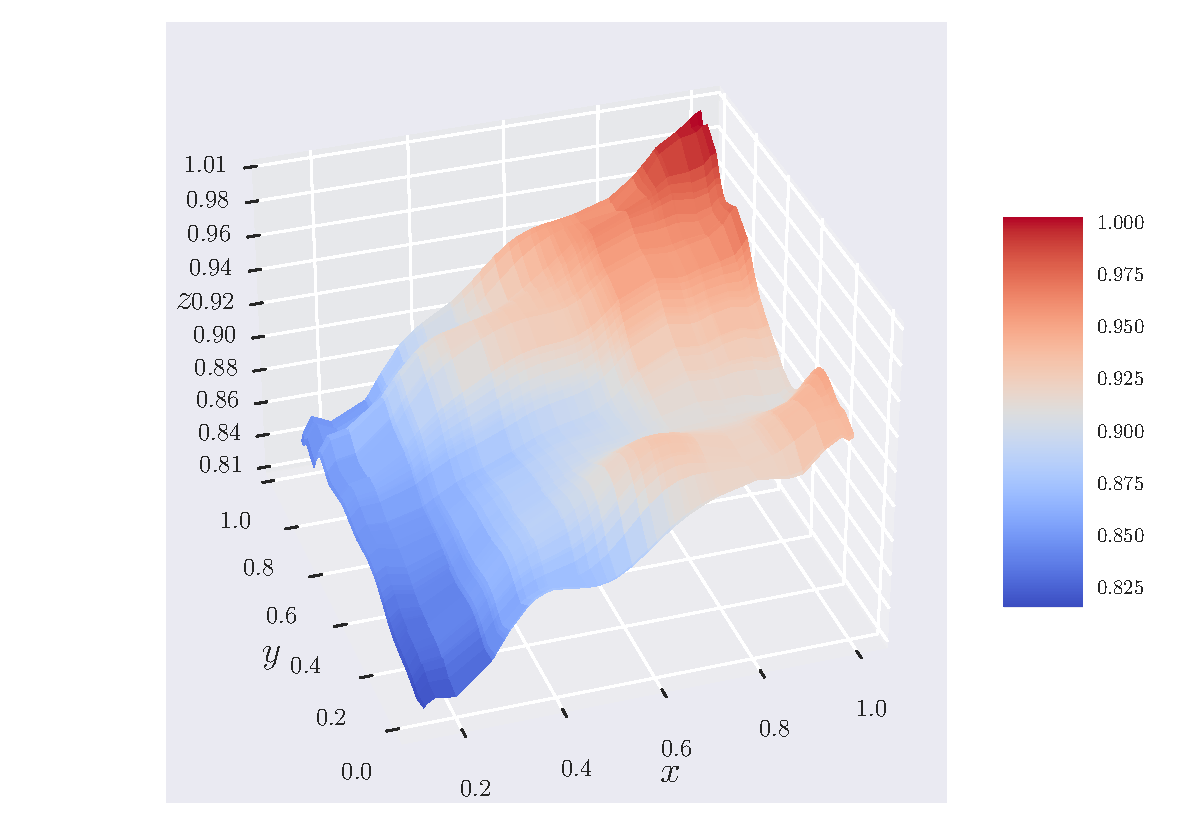
\includegraphics[width=\linewidth]{SRTM_prediction_p30.pdf}
	\endminipage\hfill
	\minipage{0.49\textwidth}
	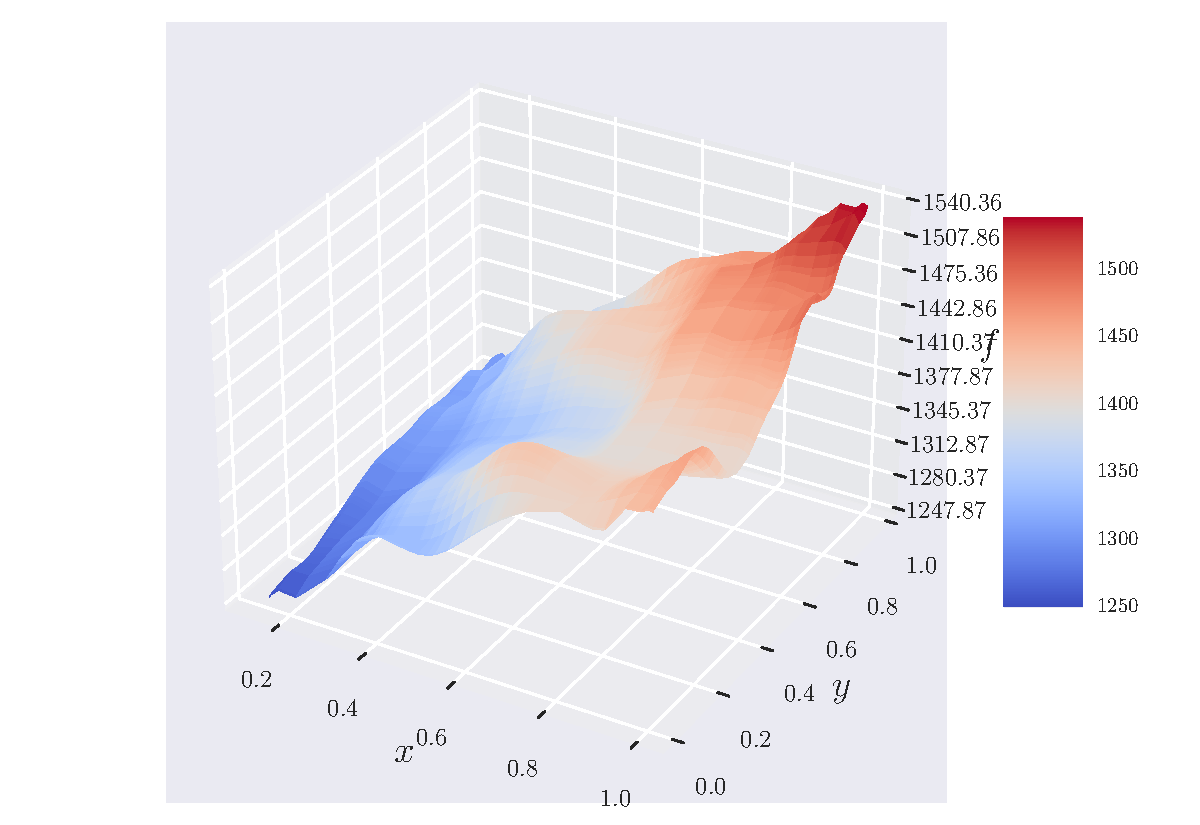
\includegraphics[width=\linewidth]{SRTM_prediction_p50.pdf}
	\endminipage
	\caption{Data til venstre. Fit til høyre}
  \label{fig:terrain_fit}
\end{figure}

In figure \ref{fig:terrain_fit} we see that $p=10$ gives a decent fit, as it captures the essential structure of the terrain. It does, however, miss out on many of the rough details in the landscape. For example the small elevation on the corner $(x,y) = (1,1)$. With $p=20$ we are able to reproduce more nuanced structures like the peak mentioned above. Increasing up to $p=30$ does not change the fit much, other than a few more details at certain points. Finally, we study the resulting fit with $p=50$. Although it provides some more rough futures of the terrain, it illustrates some difficulties of the fitting. The shape of the mountain top at $x=1$ and $y=1$ is no longer consistent with the original terrain data, and we git a tiny valley at $x=1$ and $y=0.8$, which is not an actual feature of the terrain data. Still, there are details missing along the $x$-axis at $y=1$, and the structure of the two peaks at $y=0$ is still not being represented accurately.

Next we move on to studying the MSE with cross validation. As with the bootstrap analysis, we expect the MSE to decrease in the beginning, and increase when overfitting. We use $p_\text{max} = 7$ and $k=[5,10]$ folds, and get the results shown in figure \ref{fig:terrain_OLS_MSE_CV}.

\begin{figure}[h]
	\minipage{0.49\textwidth}
	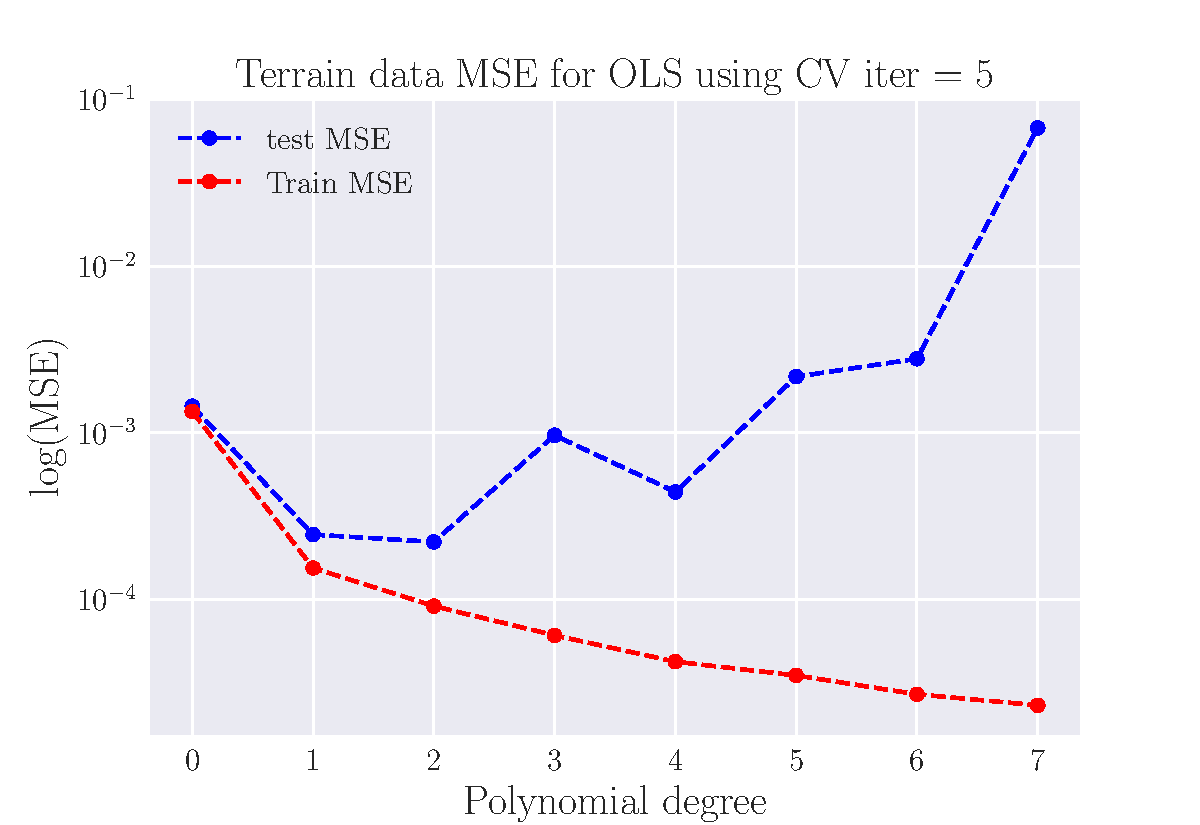
\includegraphics[width=\linewidth]{SRTM_MSE_OLS_n50_pol7_CV_re5_log.pdf}
	\endminipage\hfill
	\minipage{0.49\textwidth}
	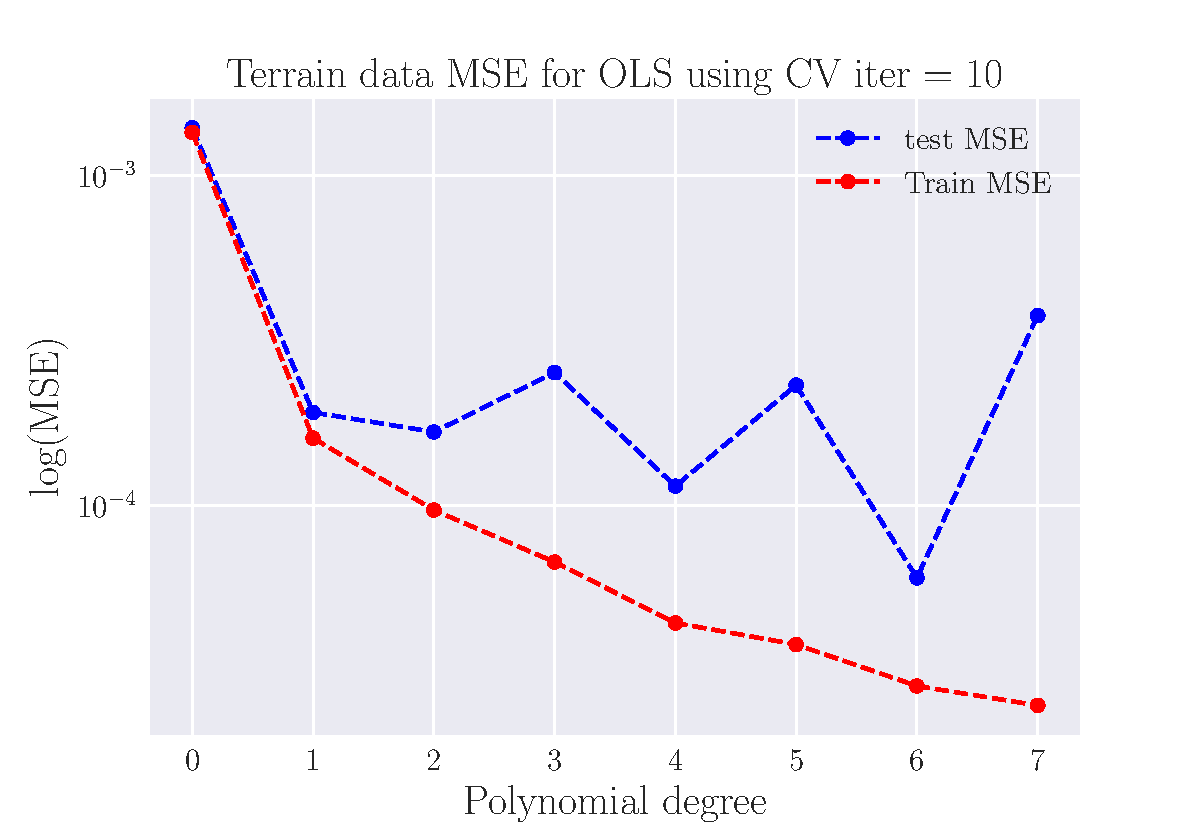
\includegraphics[width=\linewidth]{SRTM_MSE_OLS_n50_pol7_CV_re10_log.pdf}
	\endminipage
	\caption{Here we have plotted $\log(\text{MSE})$ as a function of polynomial degree, with cross-validation as the resampling technique. Left graph shows with $k=5$ iterations, and right with $k=10$.}
  \label{fig:terrain_OLS_MSE_CV}
\end{figure}
Looking at figure \ref{fig:terrain_OLS_MSE_CV} we see that the test MSE becomes large when $p>3$. Doubling the number of k-folds, the MSE drops, however the test MSE still deviates quicker, and there is a clear increase for $p>6$. With $k=10$ we seem to get a clearly increased test MSE with odd ordered polynomial degrees, a feature that was not apparent with the bootstrap method. The actual minimum $\text{MSE} \approx 2.22\cdot10^{-4}$ was found at polynomial degree $p=2$ with $k=5$ iterations. For $k=10$ we found the minimum $\text{MSE} \approx 6.05\cdot10^{-4}$ at $p=6$.

Also the MSE drops much lower in figure \ref{fig:terrain_OLS_MSE_bootstrap}, almost an order of magnitude lower. There is no clear reason as to why the results are different from those obtained when bootstrapping. One reason could be that we have an "unlucky" seed, and because we have such few resampling iterations we get deviations, just like we discussed for our Franke function results.

Now we look at bias-variance trade-off analysis, still expecting the same behavior as in exercise 2. i.e. for both test and train, the bias and MSE should start high and variance low. The train data will get a strictly better fit for higher polynomial degree, making both the bias and MSE lower. For the testing data however, when we start to see overfitting (around $p=23$) variance and error should increase, while bias stays low. Using max polynomial degree $p_\text{max}=25$ and $B=50$ iterations we get the result in figure \ref{fig:terrain_OLS_BVT}.

\begin{figure}[h]
	\minipage{0.49\textwidth}
	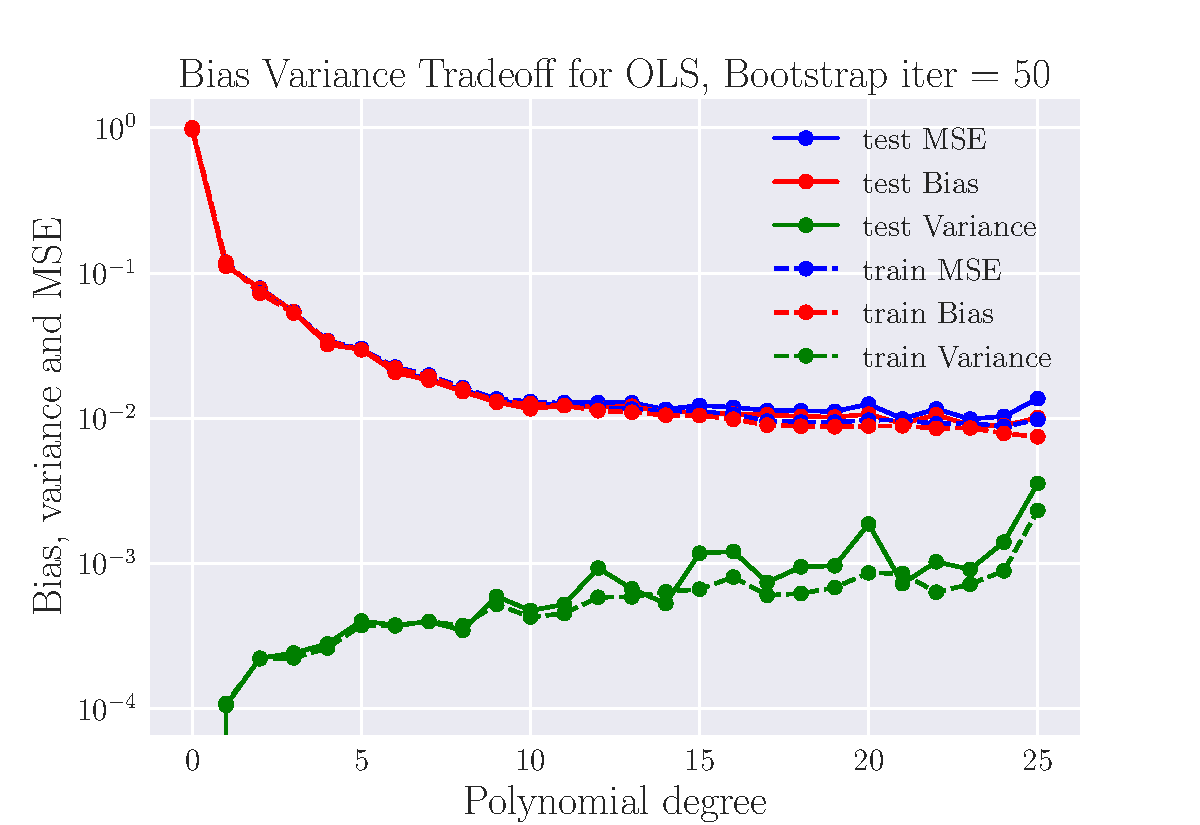
\includegraphics[width=\linewidth]{SRTM_BVT_OLS_n50_log.pdf}
	\endminipage\hfill
	\minipage{0.49\textwidth}
	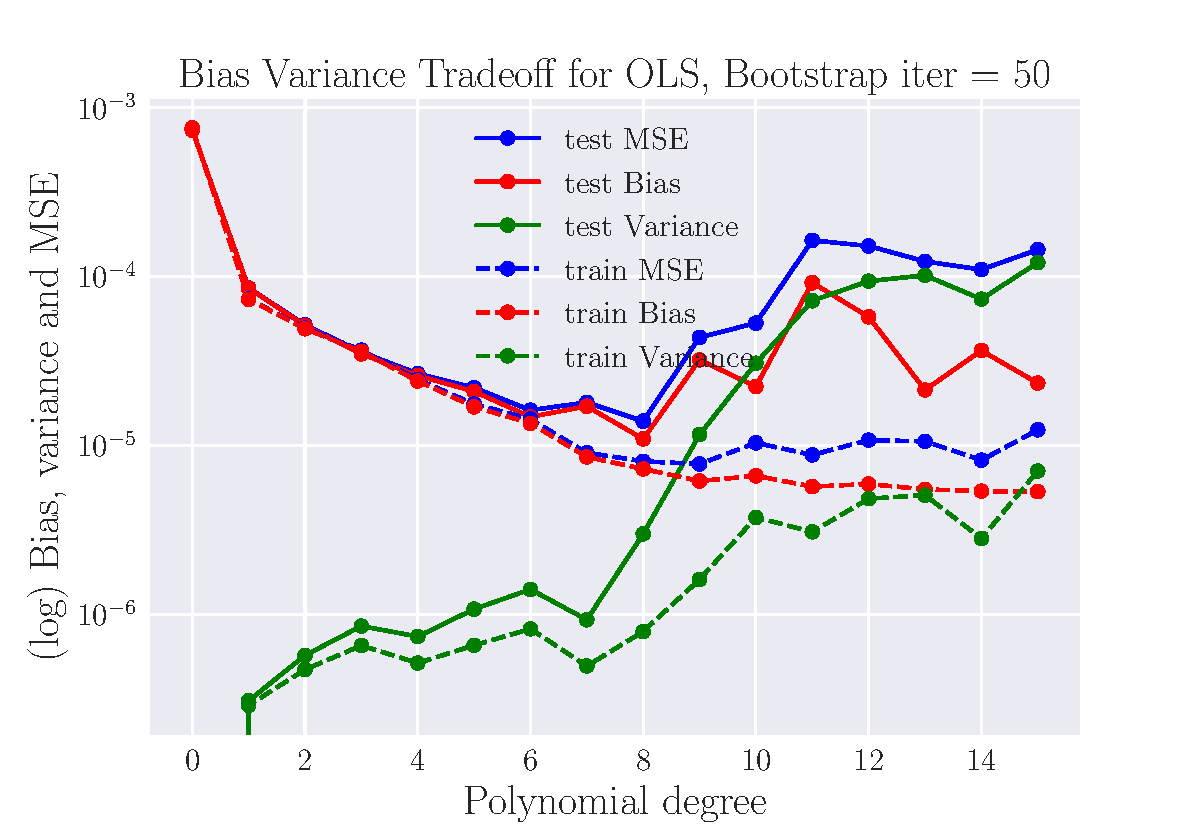
\includegraphics[width=\linewidth]{SRTM_BVT_OLS_n30_log.pdf}
	\endminipage
	\caption{Here we have plotted the logarithm of MSE, variance and bias, as a function of polynomial degree. We used $B=50$ bootstrap iterations. The left plot is with $(50\cross50)$ grid-points and right with $(30\cross30)$.}
  \label{fig:terrain_OLS_BVT}
\end{figure}

To easier see variations when we plot for $50$ data points, we use a logarithmic scale on the $y$-axis. The result is shown on the left panel in figure \ref{fig:terrain_OLS_BVT}. We see little deviations in bias and MSE, this makes sense when considering our the small MSE variations when bootstrapping (figure \ref{fig:terrain_OLS_MSE_bootstrap}). The test variance also deviates little from the train variance because of the same reason. Again for reference, we include the result obtained with fewer data points to see any noticeable effect. The bias-variance trade-off result for $15$ data points is shown on the right panel of figure \ref{fig:terrain_OLS_BVT}, up to $p=15$. This clearly shows the variations which we expect.

\subsection*{Ridge}
Next we evaluate the terrain data using Ridge regression, using bootstrap and cross validation as the resampling technique. Considering the unnoticeable variations in bias and variance in figure \ref{fig:terrain_OLS_BVT}, we omit those plots for further analysis. When using fewer datapoints, it would make more sense in including them, as we also saw in figure \ref{fig:terrain_OLS_BVT}.

Now, when we implement bootstrapping, we will use $B=90$ iterations, looking at polynomial degrees between $p_\text{min} = 8$ and $p_\text{max} = 19$, and $\lambda$-values between $10^{-2}$ and $10^{-18}$. The MSE as a function of both $\lambda$ and $p$-values is plotted in figure \ref{fig:terrain_Ridge_MSE_Boot}.
\begin{figure}[h]
	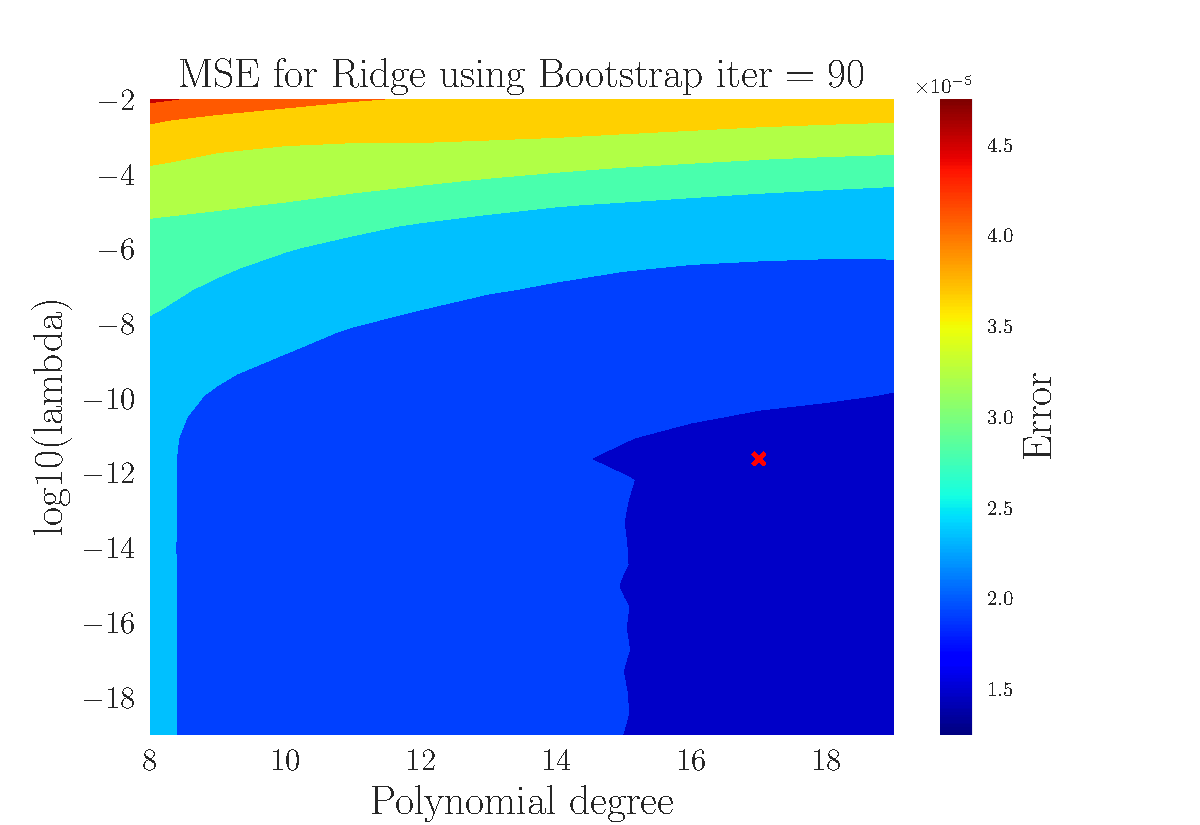
\includegraphics[width=0.8\linewidth]{SRTM_Contour_PL_Ridge_Bootstrap90_n50_eps0.2_p8_19_lmbm2_m19.pdf}
	\caption{This contour shows the MSE (colorbar), when using bootstrapping, as a function of polynomial degree ($x$-axis) and $\log(\lambda)$ ($y$-axis). The red X marks for what values of $p$ and $\lambda$ we have the minimum MSE.}
	\label{fig:terrain_Ridge_MSE_Boot}
\end{figure}
In figure \ref{fig:terrain_Ridge_MSE_Boot} we see that we get the lowest $\text{MSE} \approx 1.34\cdot10^{-5}$ (the red x) for a small $\lambda \approx 10^{-12}$ and large $p = 17$. The small $\lambda$ indicates that ordinary OLS should be a good fit. This is because when $\lambda$ shrinks, we approach OLS.

We implement cross-validation as our resampling technique. We will use 10 iterations, looking at polynomial degrees between $p_\text{min} = 1$ and $p_\text{max} = 9$, and $\lambda$-values between $10$ and $10^{-9}$. The MSE as a function of both $\lambda$ and $p$-values is plotted in figure \ref{fig:terrain_Ridge_MSE_CV}.
\begin{figure}[h]
	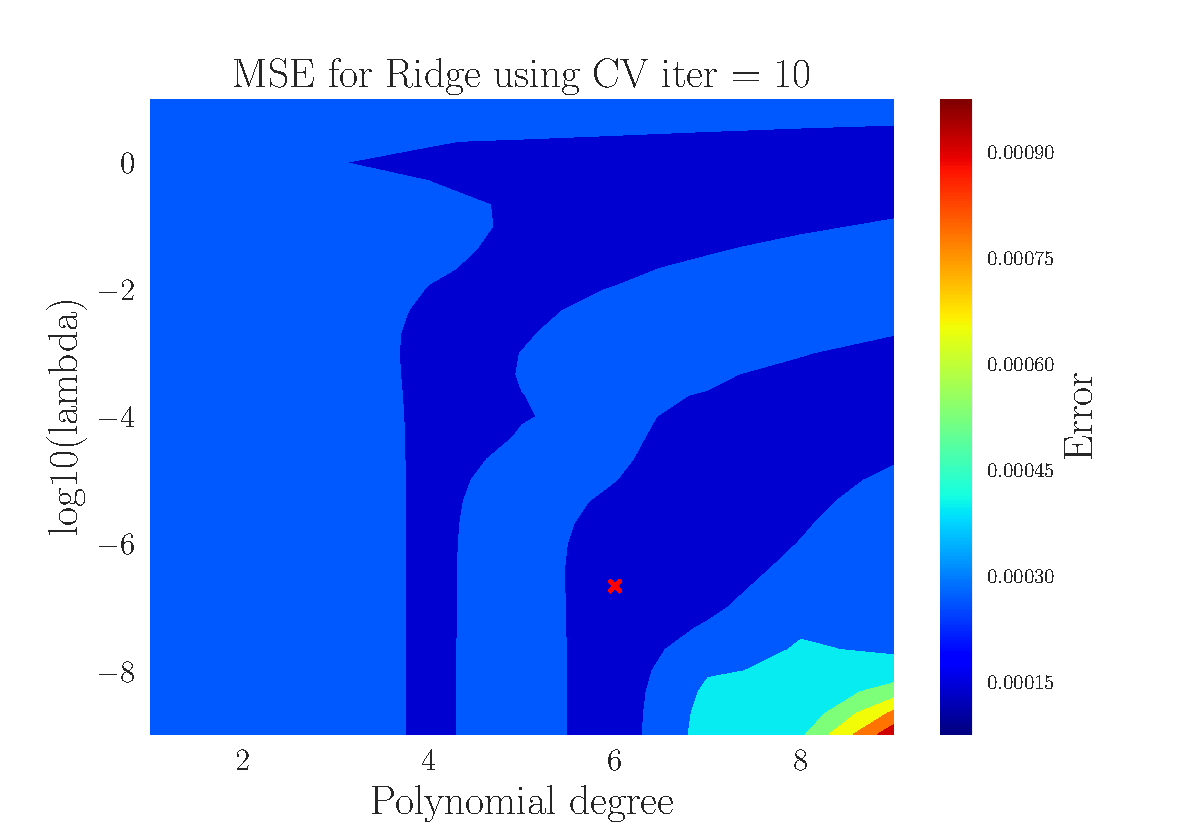
\includegraphics[width=0.8\linewidth]{SRTM_Contour_PL_Ridge_CV10_n50_eps0.2_p1_9_lmb1_m9.pdf}
	\caption{This contour shows the MSE (colorbar), when using cross-validation, as a function of polynomial degree ($x$-axis) and $\log(\lambda)$ ($y$-axis). The red X marks for what values of $p$ and $\lambda$ we have the minimum MSE.}
	\label{fig:terrain_Ridge_MSE_CV}
\end{figure}
In figure \ref{fig:terrain_Ridge_MSE_CV} we see that the lowest $\text{MSE} \approx 1.51\cdot10^{-5}$ (the red x) is with a small $\lambda \approx 10^{-7}$ and $p = 6$.

\subsection*{Lasso}
Lastly we evaluate the terrain data using Lasso regression. Here we will also implement bootstrap and cross validation as the resampling technique.  When bootstrapping, we will use $B=90$ iterations, looking at polynomial degrees between $p_\text{min} = 4$ and $p_\text{max} = 11$, and $\lambda$-values between $10^{-6}$ and $10^{-10}$. The MSE as a function of both $\lambda$ and $p$-values is plotted in figure \ref{fig:terrain_Lasso_MSE_Boot}.
\begin{figure}[h]
	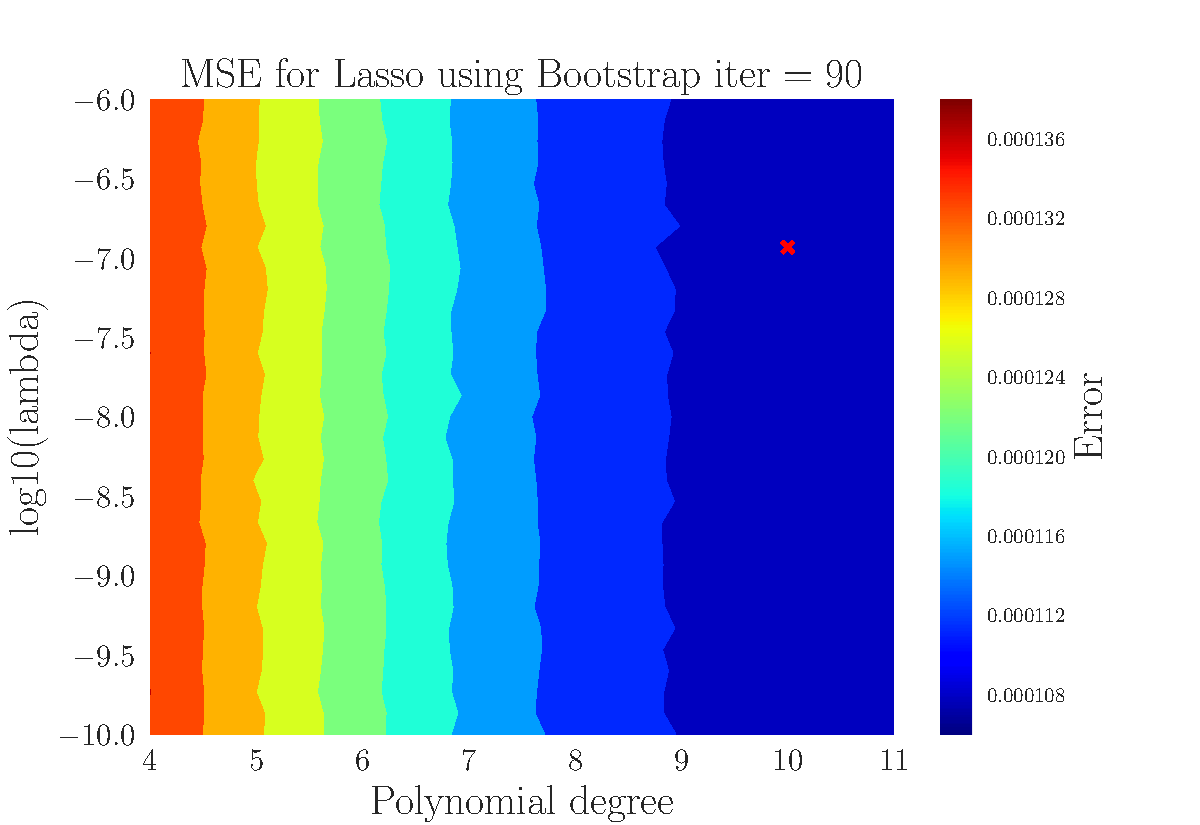
\includegraphics[width=0.8\linewidth]{SRTM_Contour_PL_Lasso_Bootstrap90_n50_eps0.2_p4_11_lmbm6_m10.pdf}
	\caption{This contour shows the MSE (colorbar), when using bootstrapping, as a function of polynomial degree ($x$-axis) and $\log(\lambda)$ ($y$-axis). The red X marks for what values of $p$ and $\lambda$ we have the minimum MSE.}
	\label{fig:terrain_Lasso_MSE_Boot}
\end{figure}
In figure \ref{fig:terrain_Lasso_MSE_Boot} we see that we get the lowest $\text{MSE} \approx 1.06\cdot10^{-4}$ (the red x) for a small $\lambda \approx 10^{-7}$ and large $p = 10$.

When we use cross-validation, we still use 10 iterations, looking at polynomial degrees between $p_\text{min} = 5$ and $p_\text{max} = 14$, and $\lambda$-values between $10^{-1}$ and $10^{-9}$. The MSE as a function of both $\lambda$ and $p$-values is plotted in figure \ref{fig:terrain_Lasso_MSE_CV}.
\begin{figure}[h]
	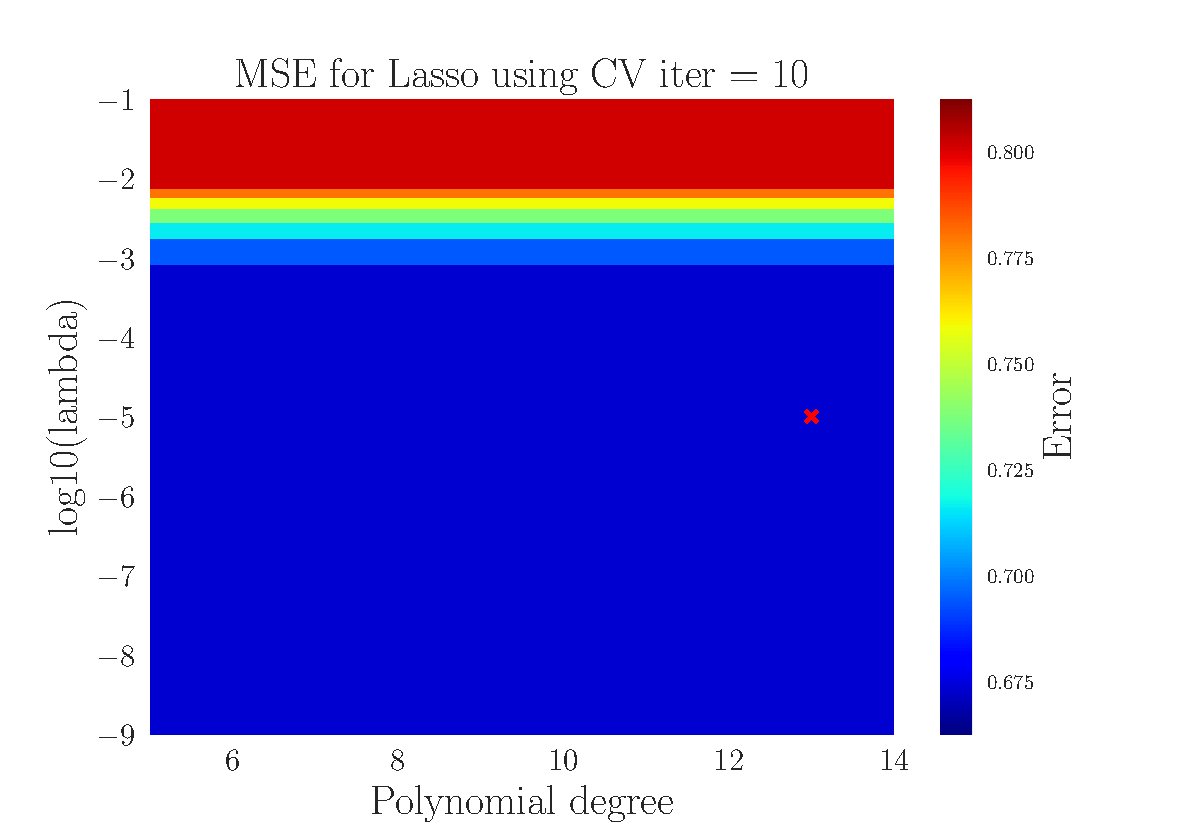
\includegraphics[width=0.8\linewidth]{SRTM_Contour_PL_Lasso_CV10_n50_eps0.2_p5_14_lmbm1_m9.pdf}
	\caption{This contour shows the MSE (colorbar), when using cross-validation, as a function of polynomial degree ($x$-axis) and $\log(\lambda)$ ($y$-axis). The red X marks for what values of $p$ and $\lambda$ we have the minimum MSE.}
	\label{fig:terrain_Lasso_MSE_CV}
\end{figure}
In figure \ref{fig:terrain_Lasso_MSE_CV} we see that the lowest $\text{MSE} \approx 0.65$ (the red x) is with $\lambda \approx 10^{-5}$ and $p = 13$.

\subsection*{Analysis}

\clearpage
\appendix

\section{Bias-variance Decomposition}\label{Apx:BVT}

We assume that our true data is generated from a noisy model with normally distributed noise $\epsilon$ with a mean of zero and standard deviation $\sigma^2$, i.e.
\begin{align*}
  \mathbf{y} &= f(\mathbf{x}) + \bm{\epsilon}
\end{align*}

We have approximated this function with our design matrix $\mathbf{X}$ and our parameters $\bm{\beta}$ such that our model becomes $\mathbf{\tilde{y}}=\mathbf{X}\bm{\beta}$, where the values of $\bm{\beta}$ were obtained by optimizing the mean squared error via the cost function, given by

\begin{align*}
  C(\mathbf{X}, \bm{\beta}) &= \frac{1}{n} \sum_{i=0}^{n-1} (y_i - \tilde{y}_i)^2 = \mathbb{E}\left[(\mathbf{y} - \mathbf{\tilde{y}})^2\right]
\end{align*}


where $\mathbb{E}$ is the expected value. % Note sample value

We want to show that the above expression can be written as
NoteNOTE: husk å definer alt, skriv i teksten hva f, y, yhat og ytilde er!

\begin{align*}
  \mathbb{E}\left[(\mathbf{y} - \mathbf{\tilde{y}})^2\right] &= \frac{1}{n} \sum_i (f_i - \expy)^2 + \frac{1}{n}\sum_i (\tilde{y}_i - \expy )^2 + \sigma^2
\end{align*}

We begin by inserting our model expression for $\mathbf{y}$ and adding and subtracting $\expy$ inside the expected value, before we square the expression.
\begin{align*}
  \mathbb{E}\bracket{(\mathbf{y} - \mathbf{\tilde{y}})^2} &= \mathbb{E}\bracket{(f(\mathbf{x}) + \bm{\epsilon} - \mathbf{\tilde{y}} - \expy + \expy)^2} = \mathbb{E}\bracket{\closed{(f(\mathbf{x}) - \expy) + \bm{\epsilon} + (\expy - \mathbf{\tilde{y}}) }^2 } \\
  &= \mathbb{E}\bracket{(f(\mathbf{x}) - \expy)^2 + \bm{\epsilon}^2 + (\expy - \mathbf{\tilde{y}})^2} \\
  &\quad+ \mathbb{E}\bracket{2\bm{\epsilon} (f(\mathbf{x}) - \expy) + 2\bm{\epsilon}(\expy - \mathbf{\tilde{y}}) + 2 (f(\mathbf{x}) - \expy)(\expy - \mathbf{\tilde{y}})}
\end{align*}

where the cross terms have been written on a separate line since the expected value is linear. Next we will focus on the cross-terms. Since $\bm{\epsilon}$ is normally distributed, it's expected value is simply the mean, which is zero in our case. The two cross terms involving $\bm{\epsilon}$ is therefore zero, so we only need to consider
\begin{align*}
  \mathbb{E}\bracket{(f(\mathbf{x}) - \expy)(\expy - \mathbf{\tilde{y}})} &= \mathbb{E}\bracket{f(\mathbf{x})\expy} - \mathbb{E}\bracket{f(\mathbf{x})\mathbf{\tilde{y}}} - \mathbb{E}\bracket{\expy\expy} + \mathbb{E}\bracket{\mathbf{\tilde{y}}\expy}
\end{align*}
Since the expected value of an expected value is just the expected value itself the last two terms in the above equation both become $\expy^2$, canceling each other out. Using that $f(\mathbf{x})$ is a deterministic function, we have $\mathbb{E}[f(\mathbf{x})]=f(\mathbf{x})$. Expressing $f(\mathbf{x})$ in terms of its expected value, we can write the first two terms in the above equation as
\begin{align*}
  \mathbb{E}\bracket{f(\mathbf{x})\expy} - \mathbb{E}\bracket{f(\mathbf{x})\mathbf{\tilde{y}}} &= \mathbb{E}\bracket{\mathbb{E}\bracket{f(\mathbf{x})}\expy} - \mathbb{E}\bracket{\mathbb{E}\bracket{f(\mathbf{x})}\mathbf{\tilde{y}}} \\
  &= \mathbb{E}\bracket{f(\mathbf{x})}\expy - \mathbb{E}\bracket{f(\mathbf{x})}\expy = 0
\end{align*}

Hence, all the cross terms in the expected value cancel out, and we're left with
\begin{align*}
  \mathbb{E}\left[(\mathbf{y} - \mathbf{\tilde{y}})^2\right] &= \mathbb{E}\bracket{\closed{f(\mathbf{x})-\expy}^2} + \mathbb{E}\bracket{\closed{\expy - \mathbf{\tilde{y}}}^2} + \mathbb{E}\bracket{\bm{\epsilon}^2}
\end{align*}

Using that $\mathbb{E}[\epsilon^2]=\sigma^2$ and writing the expected values as sums with the notation $f(\mathbf{x}_i)=f_i$, we get the desired expression. Since we have chosen $\mathbf{z}$ as our data variable we replace all the $y$ variables with $z$, yielding
\begin{align}
  \mathbb{E}\left[(\mathbf{z} - \mathbf{\tilde{z}})^2\right] &= \frac{1}{n} \sum_i (f_i - \expz)^2 + \frac{1}{n}\sum_i (\tilde{z}_i - \expz )^2 + \sigma^2
\end{align}
which is what we wanted to show.

\end{document}
